%%%---PREAMBLE---%%%%%%%%%%%%%%%%%%%%%%%%%%%%
\documentclass[twoside,12pt,final]{ucthesis-CA2012} % change this for oneside, twoside, 11pt, draft, etc.

% fix for pandoc 1.14
\providecommand{\tightlist}{%
  \setlength{\itemsep}{0pt}\setlength{\parskip}{0pt}}

%--- Packages --------------------------------------------------------
\usepackage[lofdepth,lotdepth,caption=false]{subfig}
\usepackage{fancyhdr}
\usepackage{amsmath, amssymb, graphicx}
\usepackage{xspace}
\usepackage{braket}
\usepackage{color}
\usepackage{setspace}
\usepackage{fancyvrb}
\usepackage{array}
\usepackage{ifxetex,ifluatex}
\usepackage{etoolbox}

%% for the per mil symbol
\usepackage[nointegrals]{wasysym}

%% for more attractive tables
\usepackage{booktabs}
\usepackage{xcolor}
\usepackage{longtable}
\usepackage{lscape}
\usepackage{tabularx}

\usepackage[nostamp]{draftwatermark}
% % Use the following to make modification
\SetWatermarkText{DRAFT}
\SetWatermarkLightness{0.95}

% suppress bottom page numbers on 1st page of each chapt.
% because they overlap with text
%\patchcmd{\chapter}{plain}{empty}{}{} % turn off for UCD requirements of page number on every page

%---New Definitions and Commands------------------------------------------------------

\newtheorem{theorem}{Jibberish}

\bibliography{references}

\hyphenation{mar-gin-al-ia}

% from uw_template.tex

% commands and environments needed by pandoc snippets
% extracted from the output of `pandoc -s`
%% Make R markdown code chunks work

\ifxetex
  \usepackage{fontspec,xltxtra,xunicode}
  \defaultfontfeatures{Mapping=tex-text,Scale=MatchLowercase}
\else
  \ifluatex
    \usepackage{fontspec}
    \defaultfontfeatures{Mapping=tex-text,Scale=MatchLowercase}
  \else
    \usepackage[utf8]{inputenc}
  \fi
\fi
\DefineShortVerb[commandchars=\\\{\}]{\|}
\DefineVerbatimEnvironment{Highlighting}{Verbatim}{commandchars=\\\{\}}
% Add ',fontsize=\small' for more characters per line
\newenvironment{Shaded}{}{}
\newcommand{\KeywordTok}[1]{\textcolor[rgb]{0.00,0.44,0.13}{\textbf{{#1}}}}
\newcommand{\DataTypeTok}[1]{\textcolor[rgb]{0.56,0.13,0.00}{{#1}}}
\newcommand{\DecValTok}[1]{\textcolor[rgb]{0.25,0.63,0.44}{{#1}}}
\newcommand{\BaseNTok}[1]{\textcolor[rgb]{0.25,0.63,0.44}{{#1}}}
\newcommand{\FloatTok}[1]{\textcolor[rgb]{0.25,0.63,0.44}{{#1}}}
\newcommand{\CharTok}[1]{\textcolor[rgb]{0.25,0.44,0.63}{{#1}}}
\newcommand{\StringTok}[1]{\textcolor[rgb]{0.25,0.44,0.63}{{#1}}}
\newcommand{\CommentTok}[1]{\textcolor[rgb]{0.38,0.63,0.69}{\textit{{#1}}}}
\newcommand{\OtherTok}[1]{\textcolor[rgb]{0.00,0.44,0.13}{{#1}}}
\newcommand{\AlertTok}[1]{\textcolor[rgb]{1.00,0.00,0.00}{\textbf{{#1}}}}
\newcommand{\FunctionTok}[1]{\textcolor[rgb]{0.02,0.16,0.49}{{#1}}}
\newcommand{\RegionMarkerTok}[1]{{#1}}
\newcommand{\ErrorTok}[1]{\textcolor[rgb]{1.00,0.00,0.00}{\textbf{{#1}}}}
\newcommand{\NormalTok}[1]{{#1}}
\newcommand{\OperatorTok}[1]{\textcolor[rgb]{0.00,0.44,0.13}{\textbf{{#1}}}}
\newcommand{\BuiltInTok}[1]{\textcolor[rgb]{0.00,0.44,0.13}{\textbf{{#1}}}}
\newcommand{\ControlFlowTok}[1]{\textcolor[rgb]{0.00,0.44,0.13}{\textbf{{#1}}}}

\ifxetex
  \usepackage[setpagesize=false, % page size defined by xetex
              unicode=false, % unicode breaks when used with xetex
              xetex,
              colorlinks=true,
              linkcolor=blue]{hyperref}
\else
  \usepackage[unicode=true,
              colorlinks=true,
              linkcolor=blue]{hyperref}
\fi
\hypersetup{breaklinks=true, pdfborder={0 0 0}}
\setlength{\parindent}{0pt}
\setlength{\parskip}{6pt plus 2pt minus 1pt}
\setlength{\emergencystretch}{3em}  % prevent overfull lines
\setcounter{secnumdepth}{0}

%---Set Margins ------------------------------------------------------
\setlength\oddsidemargin{0.25 in} \setlength\evensidemargin{0.25 in} \setlength\textwidth{6.25 in} \setlength\textheight{8.5 in} %8.5
\setlength\footskip{0.25 in} \setlength\topmargin{0 in} \setlength\headheight{0.25 in} \setlength\headsep{0.25 in}

%%%---DOCUMENT---%%%%%%%%%%%%%%%%%%%%%%%%%%%%
\begin{document}


%=== Preliminary Pages ============================================
\begin{ucfrontmatter}

  %%%%%%%%%%%%%%%%%%%%%%%%%%%
  % TITLE PAGE INFORMATION % % modified to meet UCDavis
  %%%%%%%%%%%%%%%%%%%%%%%%%%%

  \title{Population genetics of a sentinel stream-breeding frog (\emph{Rana
boylii})}
  \author{Ryan A Peek}
  % \prevdegreeA{B.S. (University of California, Davis) 2002}
  % \prevdegreeB{M.S. (University of San Francisco) 2010}
  \report{DISSERTATION} 
  \degree{DOCTOR OF PHILOSOPHY} 
  \degreemonth{December} \degreeyear{2018}
  \chair{Michael R. Miller}  % this is your advisor
  \othermemberA{Peter B. Moyle} % This is a member of your committee
  \othermemberB{Mark W. Schwartz} % This is a member of your committee
  \othermemberC{} % This is a member of your committee
  \numberofmembers{3} % should match the number of entries above (chair + othermembers)
  \field{Ecology}
  \campus{Davis}
	
  % MAKE THE TITLE PAGE
	\maketitle
	
	% MAKE THE APPROVAL SHEET
	% \approvalpage

  % COPYRIGHT
  % \copyrightpage % if you want
  
  % DEDICATION %
  %%%%%%%%%%%%%%%%%%%%
    \begin{dedication}

      \vspace*{20ex} % was 25
      \begin{center}
      \begin{large} % was Large

        ``\emph{The good life of any river may depend on the perception of its
        music; and the preservation of some music to perceive.}''\\
        (Aldo Leopold)
        \begin{quote}
        ``\emph{One thing to remember is to talk to the animals. If you do, they
        will talk back to you. But if you don't talk to them, they won't talk
        back to you, then you won't understand. And when you don't understand,
        you will fear, and when you fear, you will destroy the animals, and if
        you destroy the animals, you will destroy yourself}''\\
        (Chief Dan George, Tseil-Waututh Nation, North Vancouver)
        \end{quote}
      \end{large}
      \end{center}
  \end{dedication}
  % ACKNOWLEDGEMENTS %
  %%%%%%%%%%%%%%%%%%%%
  \begin{acknowledgements}
    For all the curious people who have come before and hopefully after, I
    want to acknowledge you, and I hope we can do better to inspire and
    support those voices that may not have had the opportunities or
    priviledge I have had. I am lucky to have had all I have had, and
    finishing a dissertation requires a community, and this dissertation
    would not have happened if it wasn't for the amazing community of
    family, friends, and colleagues who helped me every step of the way. In
    particular, thank you to my partner, wife and best-friend Leslie---you
    are my sun and gravity---you held me together, anchored our family, and
    made it possible to run this crazy academic ultra-marathon. To my
    dearest little tadpoles, Connor and Genevieve, you inspire me, you make
    me laugh every day, and you remind me the world still has hope as long
    as we nourish joy and curiosity. Thank you for being you, and I hope one
    day you forgive me for the amount of time I've spent staring at a
    computer. Thanks to my mom for all the support, love, and baked goods.
    Sibling, thank you for consistently inspiring me, listening to me, and
    being the best sibling one could ask for. And for all my close friends,
    bandmates, and officemates (you know who you are), you keep me sane, you
    motivate me, and you remind me every day that I really love this crazy
    journey. John, your shed and couch have probably single-handedly kept me
    anchored in ways I can't even express\ldots{}also your friendship. Thank
    you for your time, humor, and general levity. Thanks to my Dad, who has
    cajoled, pestered, and annoyed me for far too long to ``get a PhD'',
    thanks for believing it was possible even when I didn't. Also, please
    never suggest anything like this again. And to my committee and my
    colleagues at the Center for Watershed Sciences, you have all been an
    amazing resource in providing feedback, guidance, and support throughout
    my graduate student career. Finally, to my cohort and fellow students in
    the GGE, this has been a great place to grow and mature as a scientist
    and researcher. Thank you all.
  \end{acknowledgements}
  % removed CV section from this but see gauchodown or huskydown

  % ABSTRACT %
  %%%%%%%%%%%%%%%%%%%%%%%%%%%
  \begin{abstract}
    \addcontentsline{toc}{chapter}{Abstract}

    \emph{Rana boylii} is an imperiled frog species native to CA and OR, and
    it is currently designated as a species of special concern in the state
    of CA. It has been petitioned as candidate for federal (USFWS) and state
    (CDFW) listing. As a lotic breeding amphibian, \emph{R. boylii} is tied
    closely to local flow regimes in the watersheds it inhabits and is
    therefore particularly sensitive to alterations to the natural flow
    regime. Effective conservation management of this species should
    consider and prioritize maintenance of genetic diversity as part of any
    listing decision because it is closely related to the evolutionary
    capacity for adaptation to environmental change. Conservation of genetic
    diversity in this species will require several components, including
    refining potential conservation units (i.e., distinct population
    segments) and quantifying of genetic diversity and genetic diversity
    trajectories across the species range. To assess these components,
    fine-scale and landscape-scale analyses were conducted using genomic
    data from over 600 samples from 89 localities across the range of the
    species. Six genomically-distinct groups were identified, as well as
    population subdivisions at local watershed scales. One major impact on
    \emph{R. boylii} populations has been river regulation. River regulation
    has been implicated as a cause of fundamental changes to downstream
    aquatic ecosystems. Regulation changes the natural flow regime which may
    restrict population connectivity and decrease genetic diversity in some
    species. Since population connectivity and the maintenance of genetic
    diversity are fundamental drivers of long-term persistence,
    understanding the extent that river regulation impacts these critical
    attributes of genetic health is an important goal. However, the extent
    to which \emph{R. boylii} populations in regulated rivers have
    maintained connectivity and genetic diversity is unknown. The impacts of
    river regulation on \emph{R. boylii} were investigated with genomic data
    to explore the potential for long-term persistence of \emph{R. boylii}
    under continued regulation. \emph{R. boylii} in regulated rivers showed
    striking patterns of isolation and trajectories of genetic diversity
    loss relative to unregulated rivers. For example, river regulation
    explained the greatest amount of variance in population genetic
    differentiation compared with other covariates including geographic
    distance. Importantly, patterns of connectivity and genetic diversity
    loss were observed regardless of regulation level but were most
    prominent in locations with the greatest regulation intensity. Using the
    same genomic data, fine-scale analyses of \emph{R. boylii} and \emph{R.
    sierrae} in a single region of the Sierra Nevada of California was
    conducted to evaluate the potential for hybridization between species.
    Hybridization between species may combine parental genotypes in ways
    that yield reproductively sterile or isolated lineages, and
    hybridization events may be short-lived and difficult to detect. Limited
    hybridization between the species was detected in the Feather basin,
    though it appears these are terminal events based on PCA, admixture, and
    tests of heterozygosity using species diagnostic SNPs. Finally,
    rangewide quantification and comparison of genomic variation across
    populations indicates the southern coast, southern Sierra Nevada, and
    Northern Sierra/Feather basin in California should have high
    prioritization in conservation efforts due to low genomic diversity and
    trajectories of diversity loss. More broadly, these results demonstrate
    both the critical need for regional conservation in a sentinel river
    species, and the utility and power of genetic methods for assessing and
    monitoring sensitive species across many scales.

    %\abstractsignature
  \end{abstract}
  % Table of Contents %
  %%%%%%%%%%%%%%%%%%%%%%%%%%%
	\tableofcontents

\end{ucfrontmatter} % end of the preliminary pages
\begin{ucmainmatter}

\hypertarget{uw-thesis-fields}{%
\chapter{UW thesis fields}\label{uw-thesis-fields}}

Placeholder

\hypertarget{reg-health}{%
\chapter{Flow regulation associated with decreased genetic health of a
river-breeding frog species}\label{reg-health}}

\chaptermark {Flow Regulation}

\hypertarget{introduction}{%
\section{Introduction}\label{introduction}}

Rivers simultaneously connect and carve the landscapes through which
they flow. Rivers provide corridors of connectivity for riparian and
aquatic organisms such as fish, amphibians, and macroinvertebrates
(Wiens \protect\hyperlink{ref-wiens_riverine_2002}{2002}, Pringle
\protect\hyperlink{ref-pringle_what_2003}{2003}), while also acting as
physical barriers on the landscape for many terrestrial organisms
(Voelker et al. \protect\hyperlink{ref-voelker_river_2013}{2013}, Cazé
et al. \protect\hyperlink{ref-caze_could_2016}{2016}). Hydrologic
connectivity (Pringle \protect\hyperlink{ref-pringle_what_2003}{2003})
transfers energy, organisms and ultimately genetic variation and thus is
a critical component for population persistence in dynamic systems where
populations must constantly adapt to temporal and spatial changes. In
Mediterranean climates, rivers have strong seasonal patterns associated
with cold, wet winters and warm, dry summers. Native aquatic organisms
have evolved life histories well adapted to these natural patterns,
which are both predictable and seasonal (Yarnell et al.
\protect\hyperlink{ref-yarnell_ecology_2010}{2010}, Tonkin et al.
\protect\hyperlink{ref-tonkin_seasonality_2017}{2017}).

River regulation, or the hydrological alteration of flow by dams and
diversions, impacts the seasonal and interannual flow variability within
a watershed. Regulation changes the natural flow regime and dramatically
alters geomorphic and hydrologic connectivity of watersheds (Poff et al.
\protect\hyperlink{ref-poff_homogenization_2007}{2007}), which may
restrict natural population connectivity (Schick and Lindley
\protect\hyperlink{ref-schick_directed_2007}{2007}, Shaw et al.
\protect\hyperlink{ref-shaw_importance_2016}{2016}). River regulation
can change flow frequency, magnitude, duration, timing, and rate of
change, which can have significant impacts on aquatic organisms and
ecological processes (Poff et al.
\protect\hyperlink{ref-poff_homogenization_2007}{2007}, Yarnell et al.
\protect\hyperlink{ref-yarnell_ecology_2010}{2010}). River regulation,
and more specifically, regulation associated with hydropower generation,
has been implicated as a cause of fundamental changes to downstream
aquatic ecosystems (Power et al.
\protect\hyperlink{ref-power_dams_1996}{1996}, Bunn and Arthington
\protect\hyperlink{ref-bunn_basic_2002}{2002}, Moyle et al.
\protect\hyperlink{ref-moyle_rapid_2011}{2011}). The hydrological
regimes of over half of the world's largest rivers have been altered by
large dams (Nilsson et al.
\protect\hyperlink{ref-nilsson_fragmentation_2005}{2005}) and only
recently has the extent of flow alteration and the associated
ecosystem-level impacts been acknowledged (Pringle
\protect\hyperlink{ref-pringle_hydrologic_2001}{2001}, Dudgeon et al.
\protect\hyperlink{ref-dudgeon_freshwater_2006}{2006}, Murchie et al.
\protect\hyperlink{ref-murchie_fish_2008}{2008}).

Changes to abiotic processes caused by river regulation can have a
substantial impact on biotic communities. The negative effects of river
regulation on migration and loss of spawning habitat (Lind et al.
\protect\hyperlink{ref-lind_effects_1996}{1996}, Fuller et al.
\protect\hyperlink{ref-fuller_linking_2011}{2011}, Kupferberg et al.
\protect\hyperlink{ref-kupferberg_effects_2012}{2012}, Rolls and Bond
\protect\hyperlink{ref-rolls_environmental_2017}{2017}), reductions in
population abundances and diversity (Zhong and Power
\protect\hyperlink{ref-zhong_environmental_1996}{1996}, Vorosmarty et
al. \protect\hyperlink{ref-vorosmarty_global_2010}{2010}, Fuller et al.
\protect\hyperlink{ref-fuller_linking_2011}{2011}, Werth et al.
\protect\hyperlink{ref-werth_dams_2014}{2014}, Scribner et al.
\protect\hyperlink{ref-scribner_applications_2016}{2016}, Sabo et al.
\protect\hyperlink{ref-sabo_designing_2017}{2017}, Guzy et al.
\protect\hyperlink{ref-guzy_influence_2018}{2018}), and fragmentation
(Vorosmarty et al. \protect\hyperlink{ref-vorosmarty_global_2010}{2010},
Werth et al. \protect\hyperlink{ref-werth_dams_2014}{2014}, Scribner et
al. \protect\hyperlink{ref-scribner_applications_2016}{2016}, Sabo et
al. \protect\hyperlink{ref-sabo_designing_2017}{2017}, Guzy et al.
\protect\hyperlink{ref-guzy_influence_2018}{2018}) have been well
documented. However, most rivers have not been regulated for long
periods (e.g., less than 100 years) compared to the time these organisms
had to adapt to pre-anthropogenic river flow. In regulated rivers that
organisms still occupy, it remains unknown whether populations can
persist long-term with continued regulation. In other words, while some
species may have persisted since regulation began in a system (e.g.,
several decades), this does not necessarily mean these populations will
persist into the future under current flow regulation regimes. Thus,
exploring the potential for long-term persistence of populations under
different flow regimes is a crucial component for guiding conservation
efforts yet remains a significant gap.

One tool that can help address this gap is the integration of genetics
and hydrology to better assess the impact of river regulation on aquatic
organisms (Scribner et al.
\protect\hyperlink{ref-scribner_applications_2016}{2016}). Although
aquatic organisms are often difficult to count and monitor by
conventional methods, genetic monitoring can be a powerful tool to
assess population health by revealing factors such as fragmentation and
population declines. It is widely recognized that reductions in
population connectivity can increase isolation and inbreeding, leading
to a potential ``extinction vortex'' (Gilpin and Soule
\protect\hyperlink{ref-gilpin_minimum_1986}{1986}), yet there is limited
understanding of how flow alteration may impair the processes crucial
for maintenance of genetic variation and thus adaptive capacity. In
addition, there is a current pressing need for more effective and
flexible watershed management tools, particularly in relation to
monitoring aquatic populations and implementation of environmental flows
(Grantham et al. \protect\hyperlink{ref-grantham_climatic_2010}{2010}).
Thus, population genetics could be a powerful tool to understand the
influence of different flow regimes on population health and this
information could facilitate improved flow management to better protect
aquatic populations.

The river-breeding foothill yellow-legged frog (\emph{Rana boylii};
FYLF) historically occurred in lower and mid-elevation streams and
rivers from Southern Oregon to northern Baja California west of the
Sierra-Cascade crest (Stebbins
\protect\hyperlink{ref-stebbins_field_2003}{2003}). \emph{Rana boylii}
are intimately linked with river hydrology because they have evolved to
spawn in synchrony with natural flow cues associated with seasonal
spring snowmelt or rain recession periods (Kupferberg
\protect\hyperlink{ref-kupferberg_hydrologic_1996}{1996}, Yarnell et al.
\protect\hyperlink{ref-yarnell_ecology_2010}{2010},
\protect\hyperlink{ref-yarnell_management_2016}{2016}, Bondi et al.
\protect\hyperlink{ref-bondi_transferability_2013}{2013}). However,
population declines have been documented across the former range of this
species, particularly in southern California and the Sierra Nevada where
it has been extirpated from approximately 50 percent of its historical
range (Jennings and Hayes
\protect\hyperlink{ref-jennings_amphibian_1994}{1994}, Davidson et al.
\protect\hyperlink{ref-davidson_spatial_2002}{2002}).

\par

In California, particularly in the Sierra Nevada, river regulation may
be a significant environmental stressor (Lind et al.
\protect\hyperlink{ref-lind_effects_1996}{1996}, Kupferberg et al.
\protect\hyperlink{ref-kupferberg_effects_2012}{2012}). Regulated river
reaches typically alter flows by augmenting or diverting winter and
spring runoff, thereby reducing or eliminating flow cues and disrupting
natural flow regimes. Aseasonal flow fluctuation from river regulation
can scour (detach from substrate) or desiccate \emph{R. boylii} egg
masses, and the loss of clutches may have a significant demographic
impact because only one egg mass is laid per year. In many regulated
rivers in the Sierra Nevada, \emph{R. boylii} populations are now
restricted to small unregulated tributaries flowing into the regulated
mainstem.

\par

Here, we investigated the impacts of river regulation on genetic
diversity of \emph{R. boylii} populations across three different flow
regimes. Given that population connectivity and genetic diversity are
known to be play critical roles in long-term species persistence, we
explored the association between these metrics and levels of river
regulation. Our goal was to assess the genetic health (through metrics
of genetic diversity) of \emph{R. boylii} under different river
regulation regimes to better inform the potential for long-term
persistence. These data can be used to prioritize management and
conservation efforts for \emph{R. boylii}, as well as demonstrate the
potential utility of genetics for future conservation monitoring efforts
in aquatic species.

\hypertarget{methods}{%
\section{Methods}\label{methods}}

\hypertarget{ch1samplecollection}{%
\subsection{Sample collection and DNA
extraction}\label{ch1samplecollection}}

345 \emph{R. boylii} buccal or tissue samples were used in this study
across six different rivers (Table \ref{tab:CH1T1},
\protect\hyperlink{supptables}{Appendix, S1}). Field sampling was
conducted following Heyer et al.
(\protect\hyperlink{ref-heyer_measuring_1994}{1994}), under CDFW SCP
Permit \#0006881, with IACUC protocol \#19327. Individual
post-metamorphic frogs were buccal-swabbed following established
protocols (Goldberg et al.
\protect\hyperlink{ref-goldberg_frogs_2003}{2003}, Pidancier et al.
\protect\hyperlink{ref-pidancier_buccal_2003}{2003}, Broquet et al.
\protect\hyperlink{ref-broquet_buccal_2007}{2007}). Each
post-metamorphic individual was comprehensively swabbed underneath
tongue and cheek for approximately one minute. Swabs were air dried for
approximately five minutes and placed in 1.5 mL microcentrifuge tubes
while in the field. Samples were stored in the laboratory at -80°C until
DNA extraction. Where possible, tail clips from tadpole larvae were
collected, and tadpoles greater than 15 mm total length were targeted
(Wilbur and Semlitsch
\protect\hyperlink{ref-wilbur_ecological_1990}{1990}, Parris et al.
\protect\hyperlink{ref-parris_assessing_2010}{2010}). One small
(\textless{}3mm) tail clip was taken per individual tadpole and dried on
Whatman qualitative filter paper (grade 1) and stored at room
temperature. Some older tissue samples consisted of toe clips placed in
100\% ethanol for storage, and DNA extraction from these samples used
Qiagen DNeasy kits following the manufacturer's protocol. Buccal swabs
and tail clip DNA were extracted with a magnetic bead--based protocol
(Ali et al. \protect\hyperlink{ref-ali_rad_2016}{2016}) and quantified
using Quant-iT PicoGreen dsDNA Reagent (Thermo Fisher Scientific) with
an FLx800 Fluorescence Reader (BioTek Instruments).
\begin{landscape}\begin{table}

\caption{\label{tab:CH1T1}Sampling and locality information for population genomic analysis in the Yuba, Bear, and American watersheds in the northern Sierra Nevada of California, USA. The number of individuals (n) is given for the total number sequenced per location and the number of individuals that were retained after filtering across the 8,533 baits. NHD refers to the National Hydrography Dataset by USGS (U.S. Geological Survey, National Hydrography Dataset, Digital data, accessed, August 2017).}
\centering
\resizebox{\linewidth}{!}{
\begin{tabular}[t]{lrllllrrrrrrr}
\toprule
Site Name & SiteID & Locality & River & Watershed & Regulation Type & Lat. & Lon. & Elev. (m) & NHD Stream Order & NHD Total Drainage Area (sq. km) & n initial & n retained\\
\midrule
BEAR & 20 & Chicago Powerhouse & Bear & Bear & Bypass & 39.17484 & -120.8998 & 665.7990 & 4 & 136.0 & 6 & 6\\
BEAR\_GRHN & 16 & Greenhorn Creek & Bear & Bear & Bypass & 39.23206 & -120.9019 & 820.5347 & 2 & 11.0 & 15 & 6\\
BEAR\_STH2 & 19 & Steep Hollow Creek US & Bear & Bear & Bypass & 39.19444 & -120.8878 & 704.6578 & 2 & 45.0 & 7 & 6\\
BEAR\_STHA & 18 & Hawkins Ravine & Bear & Bear & Bypass & 39.18833 & -120.8981 & 706.9961 & 2 & 4.0 & 3 & 3\\
BEAR\_STHC & 17 & Steep Hollow Creek DS & Bear & Bear & Bypass & 39.20231 & -120.8754 & 736.8513 & 2 & 52.0 & 13 & 12\\
\addlinespace
MFA\_AMEC & 1 & American Canyon & MF American & American & Hydropeaking & 38.93396 & -120.9436 & 240.3928 & 2 & 9.0 & 16 & 6\\
MFA\_GASC & 2 & Gas Canyon & MF American & American & Hydropeaking & 38.96651 & -120.9325 & 241.8506 & 1 & 13.0 & 6 & 6\\
MFA\_TODC & 3 & Todd Creek & MF American & American & Hydropeaking & 38.96385 & -120.9216 & 367.7263 & 2 & 10.0 & 11 & 9\\
MFY\_OREGCK & 27 & Oregon Creek & Middle Yuba & Yuba & Bypass & 39.44188 & -121.0575 & 620.4250 & 4 & 375.0 & 15 & 13\\
MFY\_US\_OH & 28 & US Our House Dam & Middle Yuba & Yuba & Bypass & 39.41305 & -120.9903 & 624.1467 & 4 & 375.0 & 13 & 12\\
\addlinespace
NFA & 13 & Iowa Hill Mainstem & NF American & American & Unregulated & 39.11115 & -120.9168 & 386.4710 & 4 & 605.0 & 36 & 30\\
NFA\_BUNC & 8 & Bunch Canyon & NF American & American & Unregulated & 39.03762 & -120.9103 & 286.2874 & 3 & 27.0 & 15 & 14\\
NFA\_EUCH & 14 & Euchre Bar & NF American & American & Unregulated & 39.18492 & -120.7620 & 579.5186 & 4 & 508.0 & 13 & 11\\
NFA\_INDC & 10 & Indian Creek & NF American & American & Unregulated & 39.05665 & -120.9085 & 296.1071 & 2 & 24.0 & 12 & 11\\
NFA\_POND & 7 & Ponderosa Bridge & NF American & American & Unregulated & 38.99995 & -120.9406 & 240.8255 & 5 & 857.0 & 5 & 5\\
\addlinespace
NFA\_ROBR & 12 & Robbers Ravine & NF American & American & Unregulated & 39.10451 & -120.9267 & 400.0005 & 1 & 4.0 & 30 & 11\\
NFA\_SAIC & 15 & Sailor Canyon & NF American & American & Unregulated & 39.21694 & -120.4960 & 1005.5781 & 3 & 166.0 & 8 & 5\\
NFA\_SHIC & 9 & Shirttail Creek & NF American & American & Unregulated & 39.04446 & -120.8994 & 525.7589 & 4 & 141.0 & 16 & 15\\
NFA\_SLAR & 11 & Slaughter Ravine & NF American & American & Unregulated & 39.09865 & -120.9255 & 356.0791 & 2 & 6.0 & 8 & 8\\
NFMFA\_SC & 4 & NFMFA-Skunk Canyon & MF American & American & Hydropeaking & 39.02237 & -120.7369 & 521.5720 & 2 & 6.0 & 18 & 18\\
\addlinespace
NFY & 29 & Rocky Rest Mainstem & North Yuba & Yuba & Unregulated & 39.51190 & -120.9774 & 704.6863 & 5 & 669.0 & 15 & 12\\
NFY\_SLATE\_CGRAV & 30 & Slate Creek & North Yuba & Yuba & Bypass & 39.68913 & -120.9389 & 1330.9373 & 3 & 58.7 & 4 & 4\\
RUB\_LCUS & 6 & Rubicon-Long Canyon & MF American & American & Bypass & 38.98887 & -120.6900 & 415.1026 & 5 & 806.0 & 9 & 8\\
RUB\_USPH & 5 & Rubicon-US Powerhouse & MF American & American & Bypass & 38.99928 & -120.7233 & 360.5759 & 5 & 816.0 & 11 & 11\\
SFY & 26 & US Canyon Creek & South Yuba & Yuba & Bypass & 39.35386 & -120.7342 & 889.7745 & 4 & 365.0 & 6 & 6\\
\addlinespace
SFY\_LOGA & 25 & Logan Creek & South Yuba & Yuba & Bypass & 39.36914 & -120.8526 & 1201.1790 & 1 & 5.0 & 5 & 4\\
SFY\_MISC & 24 & Missouri Canyon & South Yuba & Yuba & Bypass & 39.36096 & -120.8814 & 1094.6312 & 2 & 5.0 & 8 & 6\\
SFY\_ROCKCK & 23 & Rock Creek & South Yuba & Yuba & Bypass & 39.32983 & -120.9863 & 593.5214 & 4 & 710.0 & 3 & 3\\
SFY\_SHADYCK & 21 & Shady Creek & South Yuba & Yuba & Bypass & 39.35433 & -121.0590 & 675.0255 & 2 & 15.0 & 14 & 12\\
SFY\_SPRINGCK & 22 & Spring Creek & South Yuba & Yuba & Bypass & 39.33233 & -120.9890 & 595.1054 & 3 & 24.0 & 4 & 4\\
\bottomrule
\end{tabular}}
\end{table}
\end{landscape}
\hypertarget{denovo}{%
\subsection{Sequencing and de novo assembly}\label{denovo}}

To produce a high-quality genomic resource for a frog species with a
large genome size, we first interrogated a large fraction of the genome
using a SbfI restriction enzyme and high-density RAD sequencing on an
Illumina HiSeq (Miller et al.
\protect\hyperlink{ref-miller_rapid_2007}{2007}, Baird et al.
\protect\hyperlink{ref-baird_rapid_2008}{2008}). Paired-end sequence
data were generated from 24 \emph{R. boylii} individuals collected
previously (Peek \protect\hyperlink{ref-peek_landscape_2010}{2010}) from
coastal and Sierra Nevada populations in California, USA
\protect\hyperlink{supptables}{(Appendix, S2)}. RAD libraries were
constructed following the protocol described in Ali et al.
(\protect\hyperlink{ref-ali_rad_2016}{2016}). \emph{De novo} loci
discovery and contig extension were carried via custom PERL scripts
(Miller et al. \protect\hyperlink{ref-miller_conserved_2012}{2012})
using the alignment program Novoalign and the genome assembler PRICE
(Ruby et al. \protect\hyperlink{ref-ruby_price_2013}{2013}). This
pipeline resulted in a set of 77,544 RAD contigs ranging from 300 to 800
bp which served as a \emph{de novo} partial genome reference for all
subsequent downstream analyses \protect\hyperlink{supptables}{(Appendix,
S3)}. Using these data, we filtered data to loci with 4 or fewer SNPs,
and randomly selected 10,000 loci from this subset. Using these RADSeq
data, 8,533 RAD capture baits (120bp) were designed by Arbor Biosciences
from the de novo alignment \protect\hyperlink{supptables}{(Appendix,
S4)}.

\hypertarget{rapture}{%
\subsection{Rapture sequencing}\label{rapture}}

We then performed Rapture on all study samples to identify putative
high-quality SNPs \protect\hyperlink{supptables}{(Appendix, S1)} using
RAD capture baits. Three different sequencing runs on an Illumina HiSeq
were merged together, filtered, and duplicates were removed using ANGSD
and Samtools (Li et al. \protect\hyperlink{ref-li_sequence_2009}{2009}).
Sampled individuals were aligned against the de novo partial genome
reference using the BWA-MEM algorithm (Li and Durbin
\protect\hyperlink{ref-li_fast_2010}{2010}, Li
\protect\hyperlink{ref-li_aligning_2013}{2013}) and saved to BAM format.
SAMtools was used to sort, filter for proper pairs, remove PCR
duplicates, and index binary alignment map (BAM), as well as merge
sequences from multiple libraries (Li et al.
\protect\hyperlink{ref-li_sequence_2009}{2009}).

\hypertarget{principal-component-analysis}{%
\subsection{Principal component
analysis}\label{principal-component-analysis}}

A probabilistic framework was used to discover SNPs for PCA as it does
not require calling genotypes and is suitable for low-coverage
sequencing data (Korneliussen et al.
\protect\hyperlink{ref-korneliussen_calculation_2013}{2013}, Fumagalli
et al. \protect\hyperlink{ref-fumagalli_quantifying_2013}{2013}). All
Rapture analyses were conducted using Analysis of Next Generation
Sequencing Data (ANGSD) (Korneliussen et al.
\protect\hyperlink{ref-korneliussen_angsd_2014}{2014}). ANGSD analyses
were conducted following methods from Prince et al.
(\protect\hyperlink{ref-prince_evolutionary_2017}{2017}), with a minimum
mapping quality score (\texttt{minMapQ}) of 10, a minimum base quality
score (\texttt{minQ}) of 20, and the genotype likelihood model
(\texttt{GL\ 1}) (Li \protect\hyperlink{ref-li_statistical_2011}{2011}).
To maximize data quality, samples with less than 100,000 aligned reads
were excluded \protect\hyperlink{supptables}{(Appendix, S1)} and only
sites represented in at least 50\% of the included samples
(\texttt{minInd}) were used. Settings used in ANGSD for PCA to identify
polymorphic sites included a \texttt{SNP\_pval} of
1e\textsuperscript{-6}, inferring major and minor alleles
(\texttt{doMajorMinor\ 1}), estimating allele frequencies
(\texttt{doMaf\ 2}) (Kim et al.
\protect\hyperlink{ref-kim_estimation_2011}{2011}), retaining SNPs with
a minor allele frequency of at least 0.05 \texttt{(minMaf}), genotype
posterior probabilities calculated with a uniform prior
(\texttt{doPost\ 2}), and the \texttt{doIBS\ 1} and \texttt{doCov\ 1}
options were used to generate PCA data. Principal components (PC)
summarizing population structure were derived from classic eigenvalue
decomposition and were visualized using the ggplot2 package in R (R Core
Team \protect\hyperlink{ref-r_core_team_r_2017}{2017}).

\hypertarget{genetic-differentiation-and-diversity-estimates}{%
\subsection{Genetic differentiation and diversity
estimates}\label{genetic-differentiation-and-diversity-estimates}}

Mean scaled F\textsubscript{ST} was used to quantify genetic
differentiation between populations (Wright
\protect\hyperlink{ref-wright_isolation_1943}{1943}, Rousset
\protect\hyperlink{ref-rousset_genetic_1997}{1997}). Genome-wide
F\textsubscript{ST} between population pairs was estimated by first
calculating a site frequency spectrum (SFS) for each population
(\texttt{doSaf}) (Nielsen et al.
\protect\hyperlink{ref-nielsen_snp_2012}{2012}) with ANGSD. The
two-dimensional SFS and global F\textsubscript{ST} between each
population pair were then estimated using realSFS (Korneliussen et al.
\protect\hyperlink{ref-korneliussen_angsd_2014}{2014}).
F\textsubscript{ST} was calculated between each pair of collection
locations within a watershed, and the mean of all pairwise calculations
within that watershed was calculated for each location. We calculated
the river distances (distance along river network) between locations
within watersheds using the riverdist package in R (Tyers
\protect\hyperlink{ref-tyers_riverdist_2017}{2017}), and used the mean
pairwise river distance (km) to all other locations within the
watershed. These values were plotted and a generalized linear model was
fitted (\(F_{ST}\) \textasciitilde{} \(Mean River Distance\)) in R (R
Core Team \protect\hyperlink{ref-r_core_team_r_2017}{2017}). To
calculate Watterson's \(\theta\) (\(\theta_S\)) (Watterson
\protect\hyperlink{ref-watterson_number_1975}{1975}), and Tajima's
\(\theta\) (\(\theta_\pi\)) (Tajima
\protect\hyperlink{ref-tajima_evolutionary_1983}{1983}), we used SFS
that were estimated as described above as priors (\texttt{pest}) to
calculate each statistic for each site (\texttt{doThetas}), and then
averaged to obtain a single value for each statistic (Korneliussen et
al. \protect\hyperlink{ref-korneliussen_calculation_2013}{2013}).

\hypertarget{boosted-regression-tree-modeling-of-variance-in-fst}{%
\subsection{\texorpdfstring{Boosted regression tree modeling of variance
in
F\textsubscript{ST}}{Boosted regression tree modeling of variance in FST}}\label{boosted-regression-tree-modeling-of-variance-in-fst}}

We used boosted regression tree (BRT) models with the R packages gbm
(Ridgeway \protect\hyperlink{ref-ridgeway_gbm_2015}{2015}) and dismo
(Hijmans et al. \protect\hyperlink{ref-hijmans_dismo_2017}{2017}) to
assess the relative influence of river regulation as compared to other
covariates. Boosted regression trees (BRT) are suitable frameworks for
large and complex ecological datasets because they do not assume
normality, nor linear relationships between predictor and response
variables and they ignore non-informative predictor variables (Graham et
al. \protect\hyperlink{ref-graham_influence_2008}{2008}, Steel et al.
\protect\hyperlink{ref-steel_associating_2017}{2017}). BRTs use
iterative boosting algorithms to combine simple decision trees to
improve model performance (De'ath
\protect\hyperlink{ref-death_boosted_2007}{2007}) and provide a robust
alternative to many traditional statistical methods (Phillips et al.
\protect\hyperlink{ref-phillips_maximum_2006}{2006}, Guisan et al.
\protect\hyperlink{ref-guisan_what_2007}{2007}). BRTs assess the
relative impact of modeled variables by calculating the number of times
a variable is selected for splitting a tree across all folds of the
cross validation. Following Steel et al.
(\protect\hyperlink{ref-steel_associating_2017}{2017}), estimates of
relative influence for each predictor variable were used to evaluate the
relative contribution a variable had in predicting the response. To
evaluate the relative influence of covariates on F\textsubscript{ST},
models were trained using river distance (km), elevation (m), upstream
drainage area (km2), Strahler stream order, and number of samples per
location. Stream segment data on elevation, length, slope, stream order,
and drainage area were derived from NHD Plus attributes (U.S. Geological
Survey, National Hydrography Dataset, Digital data, accessed, August
2017 at \url{http://nhd.usgs.gov/data.html}). In addition,
\(\Delta \theta\) \((\theta_\pi - \theta_S)\) was included to assess the
effect of genomic variation on F\textsubscript{ST} across regulation
types.

Model training and fitting were conducted following methods previously
described in Steel et al.
(\protect\hyperlink{ref-steel_associating_2017}{2017}). To reduce
overfitting, the learning rate (also known as the shrinking rate) was
set to 0.001. Stochastic gradient boosting was utilized to reduce
prediction error (De'ath
\protect\hyperlink{ref-death_boosted_2007}{2007}) and the fraction of
training data sampled to build each tree was 0.75, within the range as
recommended by (Brown et al.
\protect\hyperlink{ref-brown_predicting_2012}{2012}). Tree complexity
was set to three to allow for second and third order interaction
effects. The minimum number of observations required in the final nodes
of each tree was three. A ten-fold cross-validation technique allowed us
to determine the number of trees at which prediction error was minimized
using the cross-validation deviance. Model performance was evaluated
using the minimum estimated cross-validation deviance which maximized
the estimated deviance explained.

\clearpage

\hypertarget{results}{%
\section{Results}\label{results}}

\hypertarget{rapture-produces-high-quality-genomic-data-for-rana-boylii}{%
\subsection{\texorpdfstring{Rapture produces high quality genomic data
for \emph{Rana
boylii}}{Rapture produces high quality genomic data for Rana boylii}}\label{rapture-produces-high-quality-genomic-data-for-rana-boylii}}

To begin investigating the impact of river regulation on \emph{R.
boylii}, we collected frog tissue and buccal samples from 30 locations
in six rivers representing three different flow impairment levels
associated with hydropower generation. The three flow regimes assessed
were: (1) hydropeaking, where flows are pulsed on most days from late
spring through fall to provide electricity during peak-use hours and for
recreational whitewater rafting; (2) bypass, which diverts river flows
from an upstream portion of the basin to the downstream power generation
facilities; and (3) unregulated, a largely natural flow regime where no
upstream controls exist to regulate flows (Figure \ref{fig:CH1F1map}).
Flow data were obtained for each river reach using proximal USGS gaging
stations (Table \ref{tab:CH1T1}). We sampled a total of 345 \emph{R.
boylii} from sites in three major watersheds (Yuba, Bear, and American)
in the northern Sierra Nevada of California (Figure \ref{fig:CH1F1map},
Table \ref{tab:CH1T1}). The six study rivers share a similar
Mediterranean climate, underlying geology, watershed aspect
(west-slope), stream morphology (riffle-pool), and vegetative
communities, but differ in the intensity of flow regulation (Steel et
al. \protect\hyperlink{ref-steel_associating_2017}{2017}). Although
river regulation occurs in all three of the study watersheds, both the
North Yuba and North Fork (NF) American are unregulated whereas the
Middle Fork (MF) American is the only river that has a hydropeaking flow
regime (Figure \ref{fig:CH1F1map}A).
\begin{table}[!h]

\caption{\label{tab:CH1T2}Metadata for USGS gaging stations with current and historic data available for each study river}
\centering
\fontsize{11}{13}\selectfont
\begin{tabular}[t]{lllrr}
\toprule
Study Site & USGS Gage Number & Years of Record & Latitude & Longitude\\
\midrule
\addlinespace[0.3em]
\multicolumn{5}{l}{\textbf{North Yuba}}\\
\hspace{1em}North Yuba & 11413000 & 1931–Present & 39.52500 & -120.9369\\
\addlinespace[0.3em]
\multicolumn{5}{l}{\textbf{Middle Yuba}}\\
\hspace{1em}Middle Yuba & 11408550 & 1987–Present & 39.52194 & -120.5825\\
\hspace{1em}Middle Yuba & 11408700 & 1957–1966 & 39.43861 & -120.8111\\
\addlinespace[0.3em]
\multicolumn{5}{l}{\textbf{South Yuba}}\\
\hspace{1em}South Yuba & 11414250 & 1965–Present & 39.31861 & -120.6567\\
\hspace{1em}South Yuba & 11417000 & 1942–1972 & 39.36056 & -120.7706\\
\addlinespace[0.3em]
\multicolumn{5}{l}{\textbf{NF American}}\\
\hspace{1em}NF American & 11427000 & 1942–Present & 38.93611 & -121.0228\\
\addlinespace[0.3em]
\multicolumn{5}{l}{\textbf{Rubicon}}\\
\hspace{1em}Rubicon & 11433200 & 1959–1984 & 38.99250 & -120.7206\\
\hspace{1em}Rubicon & 11427765 & 1974–Present & 39.00027 & -120.7231\\
\addlinespace[0.3em]
\multicolumn{5}{l}{\textbf{MF American}}\\
\hspace{1em}MF American & 11433300 & 1958–2011 & 39.00611 & -120.7597\\
\hspace{1em}MF American & 11433500 & 1911–1986 & 38.91805 & -121.0142\\
\hspace{1em}MF American & OXB (PCWA)\textsuperscript{1} & 1997–Present & 39.00600 & -120.7600\\
\bottomrule
\multicolumn{5}{l}{\textsuperscript{1} PCWA=Placer County Water Agency, http://cdec.water.ca.gov/cdecstation2/?sta=OXB}\\
\end{tabular}
\end{table}







\begin{figure}
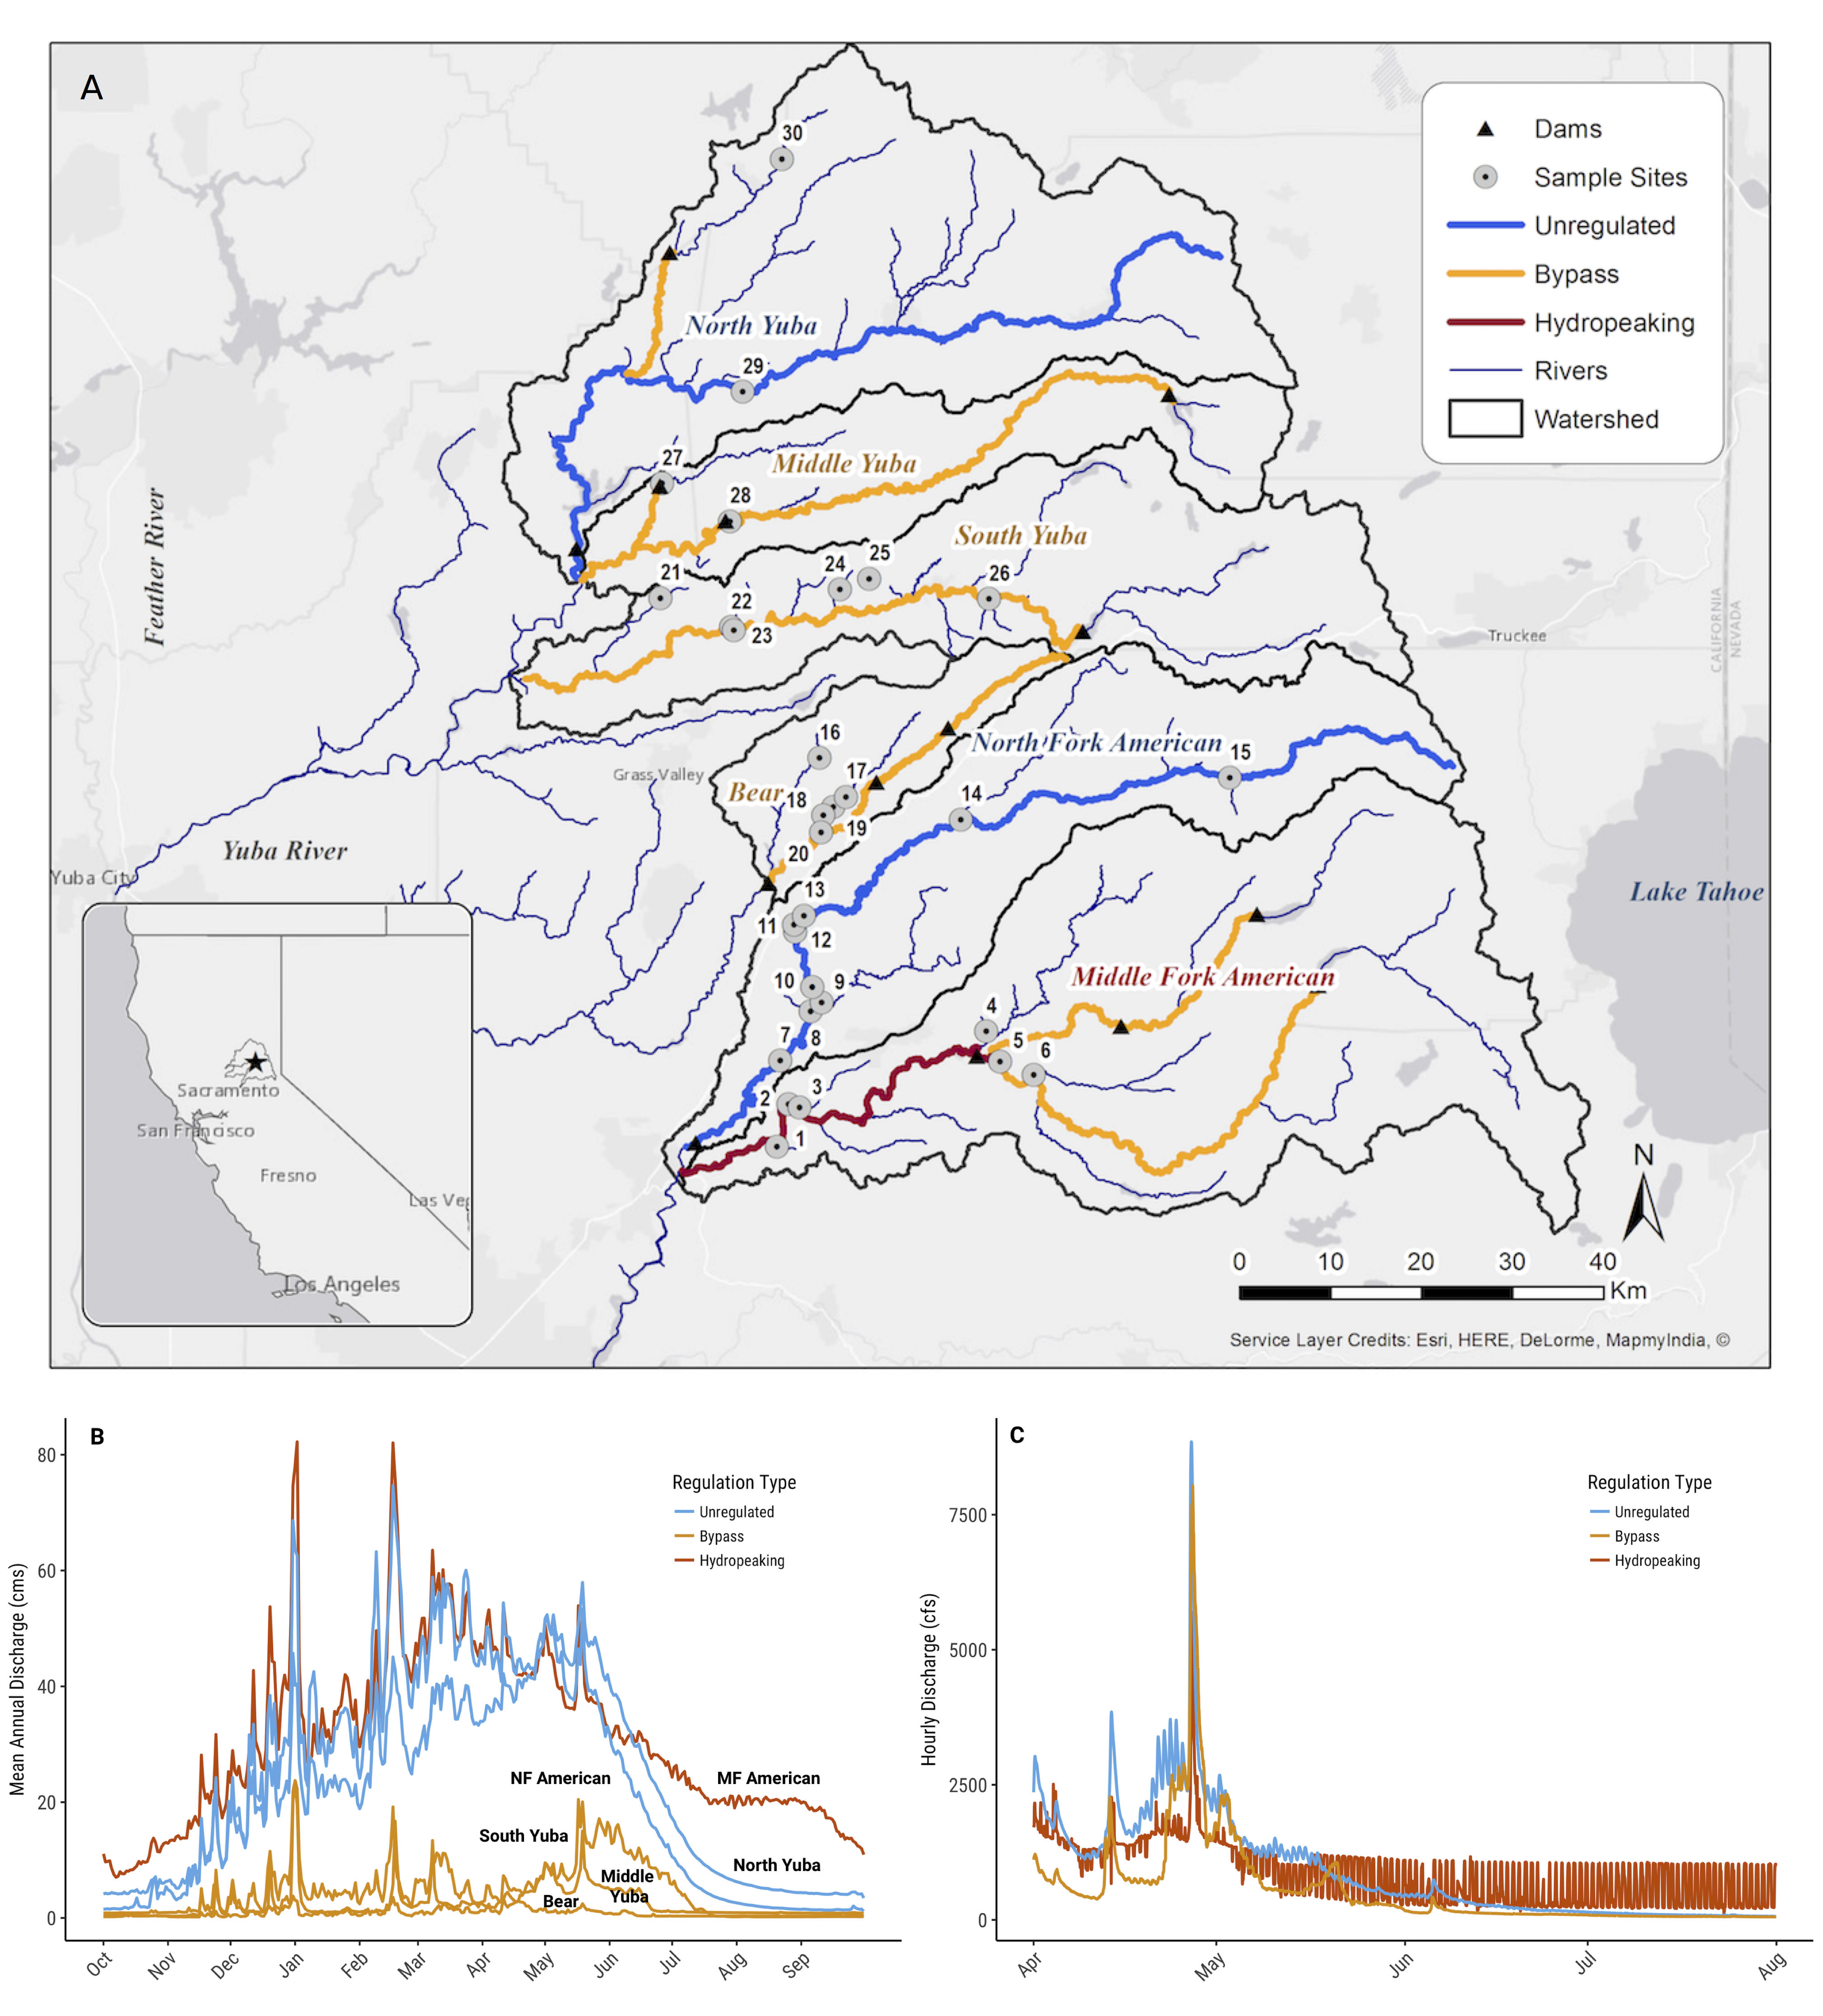
\includegraphics[width=1\linewidth]{figure/ch1/fig_01_ac_map_hydrographs} \caption{Sampling locations and flow characteristics. A) Map of
sampling locations spread across six rivers. B) Comparison of annual
mean daily discharge from 1981--2016 for three flow types. C) Comparison
of hourly discharge in three different flow regimes in April through
July 2012, Bypass (South Yuba), Hydropeaking (Middle Fork American), and
Unregulated (North Fork American). See Table \ref{tab:CH1T2} for USGS
gaging station information.}\label{fig:CH1F1map}
\end{figure}
To generate genetic data from the samples, we performed RAD Capture
(a.k.a. Rapture) (Ali et al. \protect\hyperlink{ref-ali_rad_2016}{2016})
on the samples by generating SbfI RAD libraries, capturing a subset of
the RAD loci using 8,533 baits (see Methods), and sequencing the
resulting library on an Illumina HiSeq. We then aligned the sequencing
reads from each sample to a de novo RAD assembly (see Methods). The mean
number of filtered alignments across all 345 samples was 324,928. For
downstream analysis, we selected individuals that had greater than
100,000 alignments (n=277), which provided sufficient data to
investigate population genetic attributes at broad and fine geographic
scales (see below). \emph{R. boylii} are cryptic, and often occur in low
densities within the study area. Thus, we retained a minimum of three
individuals per site, and the mean number of samples per site was
approximately nine (Table \ref{tab:CH1T1}). With genomic data,
population genetic parameters can be accurately estimated from even low
sample numbers (Hotaling et al.
\protect\hyperlink{ref-hotaling_demographic_2018}{2018}), and genomic
analyses in non-model organism often use fewer loci (Narum et al.
\protect\hyperlink{ref-narum_genotyping-by-sequencing_2013}{2013}). We
conclude that the sequence data we obtained should be appropriate for
population genetic analyses across our study area.

\hypertarget{anomalous-genetic-pattern-in-highly-regulated-reach-of-middle-fork-american-watershed}{%
\subsection{Anomalous genetic pattern in highly regulated reach of
Middle Fork American
watershed}\label{anomalous-genetic-pattern-in-highly-regulated-reach-of-middle-fork-american-watershed}}

To assess \emph{R. boylii} population structure across the collection
locations, we used ANGSD (Korneliussen et al.
\protect\hyperlink{ref-korneliussen_angsd_2014}{2014}) to discover
44,406 SNPs and perform principal component analysis (PCA; see Methods),
which provides a dimensionless comparison of all samples. The first two
principal components revealed four main groups corresponding to the
Yuba, Bear, North Fork (NF) American, and Middle Fork (MF) American
samples (Figure \ref{fig:CH1F2pca}A). Unlike the Yuba watershed where
all rivers clustered as one group, the two rivers within the American
watershed (the NF American and MF American) were separated by both PC1
and PC2. Although the NF American watershed clustered closely with the
adjacent Bear watershed, the MF American showed a surprisingly high
degree of genetic differentiation from other locations (Figure
\ref{fig:CH1F2pca}A). These data suggest that there is less genetic
differentiation between the NF American and the Bear watersheds, than
between the NF and MF American watersheds. We conclude that measurements
of overall genetic differentiation in \emph{R. boylii} from our study
area largely conform to watershed and geographic expectations, with the
exception of the American watershed, which shows a surprisingly high
degree of genetic differentiation between the North (unregulated) and
Middle (hydropeaking) Forks.




\begin{figure}
\includegraphics[width=1\linewidth]{figure/ch1/fig_02_pca_combined_v2} \caption{Principal component analysis of Rapture sequencing
data. A) Northern Sierra Nevada (n=277) watersheds and regulation types;
B) Unregulated NF American; C) and D) Hydropeaking MF American Reach.}\label{fig:CH1F2pca}
\end{figure}
To further investigate patterns of genetic variation within the American
watershed, we performed two PCAs, one on samples from the NF American,
and the other on samples from the MF American. The PCA of the NF
American showed minimal differentiation among locations, with different
study sites blending together and weak patterns of population structure
(Figure \ref{fig:CH1F2pca}B). In contrast, PCA of the MF American showed
strong differentiation between sites (Figures \ref{fig:CH1F2pca}C,
\ref{fig:CH1F2pca}D). The MF American PCA completely resolved all sites,
with the first component (PC1) strongly differentiating the samples in
the hydropeaking reach from all other sites in the MF American. This
pattern may be due to the differential river regulation between the two
rivers; the NF American is unregulated and has weak PCA differentiation,
whereas the MF American has a higher level of river regulation and all
sites form distinct genetic clusters, indicative of reduced gene flow
among sites within the MF American.

\hypertarget{river-regulation-is-the-strongest-predictor-of-genetic-isolation-with-r.-boylii-in-the-northern-sierra}{%
\subsection{\texorpdfstring{River regulation is the strongest predictor
of genetic isolation with \emph{R. boylii} in the Northern
Sierra}{River regulation is the strongest predictor of genetic isolation with R. boylii in the Northern Sierra}}\label{river-regulation-is-the-strongest-predictor-of-genetic-isolation-with-r.-boylii-in-the-northern-sierra}}

To assess how patterns of genetic differentiation are associated with
river regulation across our entire study area, we estimated pairwise
F\textsubscript{ST} (Wright
\protect\hyperlink{ref-wright_isolation_1943}{1943}) between all
collection locations within a river for all six rivers. We then plotted
the scaled mean pairwise F\textsubscript{ST} {[}mean F\textsubscript{ST}
/ (1-mean F\textsubscript{ST}){]} (Rousset
\protect\hyperlink{ref-rousset_genetic_1997}{1997}) for each location
against the mean river distance (the average distance along the river
network from each collection location to every other location within
that study river). Furthermore, each location was categorized by
regulation level of closest mainstem location. While there was a clear
relationship between F\textsubscript{ST} and river distance (as shown by
the slope of regression lines in Figure \ref{fig:CH1F3fst}A), there was
a striking pattern of elevated F\textsubscript{ST} by regulation type
(Figure \ref{fig:CH1F3fst}A). Even the bypass regulation type showed a
distinct pattern of elevated F\textsubscript{ST} compared to the
unregulated type. For instance, regulated rivers with locations
separated by less than 10km had F\textsubscript{ST} values comparable to
unregulated locations separated by mean river distances over 30 km.
Hydropeaking was the most extreme pattern of the three regulation types
and showed highly elevated F\textsubscript{ST} values with the steepest
regression coefficient. The baseline F\textsubscript{ST} or global mean
increased by over 0.1 between the unregulated (mean
F\textsubscript{ST}=0.141), and regulated locations (global mean for
bypass F\textsubscript{ST}=0.256, hydropeaking
F\textsubscript{ST}=0.278). This suggests a greater degree of isolation
within sites in regulated river reaches compared with \emph{R. boylii}
populations in unregulated reaches, as larger F\textsubscript{ST} values
represent reductions in heterozygosity due to population subdivision
(Slatkin \protect\hyperlink{ref-slatkin_gene_1987}{1987}). We conclude
\emph{R. boylii} in regulated rivers show patterns of greater population
isolation and loss of heterozygosity compared to frogs in unregulated
locations.

To investigate the relative influence of river regulation compared to
other covariates such as river distance on genetic differentiation
(i.e.~F\textsubscript{ST}), we used boosted regression tree (BRT)
modeling. Covariates included flow regime alteration type, river
distance, watershed variables derived from National hydrology data
(NHD), topographic data, and allele frequency spectrum skew. We found
flow regulation explained the greatest amount of variance in
F\textsubscript{ST} (Figure \ref{fig:CH1F3fst}B). Thus, river regulation
has a larger relative influence than mean river distance between
sampling locations, which is often the most important factor influencing
genetic differentiation (Wright
\protect\hyperlink{ref-wright_isolation_1943}{1943}, Slatkin
\protect\hyperlink{ref-slatkin_gene_1987}{1987}, Rousset
\protect\hyperlink{ref-rousset_genetic_1997}{1997}). We conclude there
is a pattern of isolation and limited connectivity between populations
in regulated reaches.






\begin{figure}
\includegraphics[height=0.6\textheight]{figure/ch1/fig_03ab_fst_brt_cowplot_for_phd} \caption{Relationship between river regulation and genetic
differentiation in \emph{R. boylii}. A) Mean pairwise
F\textsubscript{ST} vs.~mean river distance for each location; B)
Relative influence of variables on F\textsubscript{ST} from boosted
regression tree models.}\label{fig:CH1F3fst}
\end{figure}
\clearpage

\hypertarget{river-regulation-strongly-correlated-with-decreasing-genetic-diversity-in-r.-boylii}{%
\subsection{\texorpdfstring{River regulation strongly correlated with
decreasing genetic diversity in \emph{R.
boylii}}{River regulation strongly correlated with decreasing genetic diversity in R. boylii}}\label{river-regulation-strongly-correlated-with-decreasing-genetic-diversity-in-r.-boylii}}

To investigate the association between river regulation and genetic
diversity trajectory (stable, increasing, or decreasing), we summarized
patterns of genetic variation using two estimators of \(\theta\)
(\(4N\mu\)): Tajima's \(\theta\) (\(\theta_\pi\)) is based on the
average number of pairwise differences (Tajima
\protect\hyperlink{ref-tajima_evolutionary_1983}{1983}) and Watterson's
\(\theta\) (\(\theta_S\)) is based on the number of segregating sites
(Watterson \protect\hyperlink{ref-watterson_number_1975}{1975}). These
estimators are influenced by the demographic history of a population and
provide information on the trajectory of changes in genetic diversity.
When genetic diversity has been stable, these estimates are generally
equal; but when genetic diversity has been increasing,
\(\theta_\pi > \theta_S\); and when genetic diversity has been
decreasing, \(\theta_S > \theta_\pi\). We found zero populations sampled
within regulated watersheds had evidence of increasing genetic diversity
(e.g., a \(\theta_\pi - \theta_S\) that was less than zero) (Figure
\ref{fig:CH1F4theta}A). The regulated locations showed a clear
trajectory of genetic diversity loss (Figure \ref{fig:CH1F4theta}A,
\ref{fig:CH1F4theta}B). Three of the four hydropeaking locations had the
highest values of \(\Delta\theta\) (\(\theta_\pi - \theta_S\)), and the
global mean was significantly different from other regulation types.
Although some tributary populations within unregulated watersheds also
showed signs of genetic diversity loss, the mean genetic diversity
trajectory at unregulated locations was largely neutral (Figure
\ref{fig:CH1F4theta}B). This indicates populations in the northern
Sierra Nevada which are already limited in number are losing genetic
variation, and river regulation appears to be exacerbating these
patterns. We conclude there is evidence of recent genetic diversity loss
across populations in the regulated river systems, regardless of
regulation type.










\begin{figure}
\includegraphics[height=0.8\textheight,scale=1.1]{figure/ch1/fig_04ab_theta_combined_for_phd} \caption{Relationship between river regulation and genetic
diversity trajectory in \emph{R. boylii}. A) Assessment of genetic
diversity trajectories using \(\Delta\theta\)
(\(\theta_\pi - \theta_S\)) for each sampling location; B) Boxplots of
difference between \(\theta_\pi - \theta_S\) and pairwise significance
between regulation groups using a pairwise Wilcoxon rank sum test with
bonferroni correction (P \textless{} 0.05). Negative values represent
trends of increasing genetic diversity, positive values represent
trajectories of diversity loss, values near zero are stable.}\label{fig:CH1F4theta}
\end{figure}
\clearpage

\hypertarget{discussion}{%
\section{Discussion}\label{discussion}}

Although massive parallel sequencing (MPS) technologies have the
potential to facilitate collection of high-quality genetic data in
virtually any species, a number of challenges still remain for many
species including low quality or non-existent reference genomes,
large/complex/repetitive genomes, and high cost of processing/sequencing
in studies with many samples. Amphibians are particularly challenging as
many species have very large genome sizes (Nunziata et al.
\protect\hyperlink{ref-nunziata_genomic_2017}{2017}), for example, there
are only two frog reference genome assemblies available as of 2018
(Hellsten et al. \protect\hyperlink{ref-hellsten_genome_2010}{2010}, Sun
et al. \protect\hyperlink{ref-sun_whole-genome_2015}{2015}). Our results
demonstrate that Rapture (Ali et al.
\protect\hyperlink{ref-ali_rad_2016}{2016}) is a suitable method to
rapidly and inexpensively discover a large number of loci in a frog
species with a complex genome. In this study, we used new RAD sequencing
and RAD capture (Rapture) methods (Ali et al.
\protect\hyperlink{ref-ali_rad_2016}{2016}) to generate high-quality
genomic data suitable for discovering and genotyping many single
nucleotide polymorphisms (SNPs) in \emph{R. boylii}. Based on this
dataset, we were able to successfully characterize patterns of genetic
variation within \emph{R. boylii} as well as design a set of RAD capture
baits that can be used as a genetic monitoring resource for \emph{R.
boylii} (and likely other ranid species). This highlights that the
collection of genetic information, even from large numbers of samples or
in complex genomes, is no longer a limitation with current genomic
methods such as RAD and Rapture.

Demographic connectivity is widely recognized as a fundamental driver of
long-term population persistence (Fahrig and Merriam
\protect\hyperlink{ref-fahrig_habitat_1985}{1985}, Taylor et al.
\protect\hyperlink{ref-taylor_connectivity_1993}{1993}). Populations
must adapt over time and connectivity is a major way to transfer genetic
information. For example, previous studies have shown that adaptation
can occur by spreading specific alleles across large geographic
distances (Miller et al.
\protect\hyperlink{ref-miller_conserved_2012}{2012}, Prince et al.
\protect\hyperlink{ref-prince_evolutionary_2017}{2017}). In many
regulated river reaches in the Sierra Nevada, \emph{R. boylii} now occur
in isolated locations, breeding in tributaries rather than mainstem
habitats. However, since these frogs have the potential to move long
distances (Bourque (\protect\hyperlink{ref-bourque_spatial_2008}{2008})
documented \emph{R. boylii} individuals that moved over 1 km in a day),
the extent to which current population connectivity has been lost due to
river regulation remains unknown. Examining pairwise
F\textsubscript{ST}, revealed a major decrease in connectivity in
populations in regulated systems, even with limited river regulation
(i.e., bypass reaches). Usually isolation by distance patterns best
describe variation in genetic data, yet the primary factor influencing
genetic differentiation among these rivers is hydrologic alteration
(Figure \ref{fig:CH1F3fst}B). Thus, despite being able to move long
distances, \emph{R. boylii} have not been able to maintain population
connectivity in regulated rivers. This demonstrates that even in species
that can move relatively long distances and pass potential physical
barriers (e.g., infrastructure such as dams, canals, and reservoirs
likely do not represent true barriers to movement of \emph{R. boylii}),
loss of connectivity may still occur and can be revealed with genetic
analysis.

Genetic diversity is also a critical component for long-term population
persistence because it is closely related to the evolutionary capacity
for adaptation to environmental changes (Lande and Shannon
\protect\hyperlink{ref-lande_role_1996}{1996}, Frankham
\protect\hyperlink{ref-frankham_introduction_2002}{2002}, Hoffmann and
Sgrò \protect\hyperlink{ref-hoffmann_climate_2011}{2011}, Ishiyama et
al. \protect\hyperlink{ref-ishiyama_differential_2015}{2015}). In some
cases, isolated populations can maintain genetic diversity when they are
sufficiently sized (Whiteley et al.
\protect\hyperlink{ref-whiteley_genetic_2010}{2010}), however, species
of conservation concern typically have small and/or declining
populations and thus may be susceptible to genetic diversity loss (Krohn
et al. \protect\hyperlink{ref-krohn_conservation_2018}{2018}).
Throughout the Sierra Nevada, \emph{R. boylii} have largely disappeared
from regulated mainstem rivers, but the extent to which existing
populations have been able to maintain genetic diversity is unclear.
Strikingly, our analysis revealed that every single population within
the regulated watersheds exhibits a trajectory of genetic diversity
loss. Thus, genomic analysis of molecular variation provides a powerful
lens to discover and assess trajectories of genetic diversity.

Our analyses, using metrics that can serve as a reasonable proxy for
genetic health of a population, does not bode well for the long-term
persistence of \emph{R. boylii} populations in regulated rivers in the
Sierra Nevada. Many of these \emph{R. boylii} populations are already
losing genetic diversity and given their small size and reduced
connectivity the effects of inbreeding will likely exacerbate their
problems. \emph{Rana boylii} have evolved in river systems with
consistent hydrologic seasonality and predictability, despite
inter-annual variation. Flow regulation has altered patterns of
hydrologic seasonality and predictability in many watersheds (Kupferberg
et al. \protect\hyperlink{ref-kupferberg_effects_2012}{2012}). Long-term
population persistence may still be possible if conservation efforts
utilize methods that promote or maintain genetic diversity and increase
population connectivity. For example, simulations by Botero et al.
(\protect\hyperlink{ref-botero_evolutionary_2015}{2015}) demonstrated
adaptation persisted in modeled populations through large environmental
changes---if phenotypic strategies were appropriate before and after the
change---but modeled populations declined rapidly when the current
strategy was a mismatch to the current environment. Thus, \emph{R.
boylii} conservation efforts should focus on river reaches where flow
management may provide opportunities to more closely mimic local natural
flow regimes and improve hydrologic connectivity to prevent further
genetic diversity loss.

\hypertarget{conclusion}{%
\section{Conclusion}\label{conclusion}}

Detecting evolutionary responses to within- and among-year changes in an
ecological or hydrological context has previously been difficult.
However, utilizing genetic data can fill these gaps and provide a highly
informative process for identifying the impacts of anthropogenic and
environmental change on the process of adaptation (Kahilainen et al.
\protect\hyperlink{ref-kahilainen_conservation_2014}{2014}, Botero et
al. \protect\hyperlink{ref-botero_evolutionary_2015}{2015}). We
demonstrate that an aquatic species that has adapted to local hydrology
patterns shows poor genetic health (i.e., clear patterns of decreased
connectivity and trajectories of genetic diversity loss). Our results
highlight the potential impact of river regulation on aquatic organisms
and their potential for long term persistence. In the future, similar
genetic approaches could be used in many other contexts to explore the
impacts of river regulation on aquatic organisms. Taken together, our
results demonstrate that genetic monitoring can be a powerful tool for
assessment of population health and should be a critical component of
conservation management in aquatic organisms.

\hypertarget{hybrids}{%
\chapter{Hybridization between two sympatric ranid frog species in the
northern Sierra Nevada, California}\label{hybrids}}

Placeholder

\hypertarget{introduction-1}{%
\section{Introduction}\label{introduction-1}}

\hypertarget{methods-1}{%
\section{Methods}\label{methods-1}}

\hypertarget{ch2samplecollection}{%
\subsection{Sampling and DNA Extraction}\label{ch2samplecollection}}

\hypertarget{rapture2}{%
\subsection{Rapture Sequencing}\label{rapture2}}

\hypertarget{pca-and-admixture}{%
\subsection{PCA and Admixture}\label{pca-and-admixture}}

\hypertarget{f1vsf2}{%
\subsection{F1 vs.~F2 Test with Species Diagnostic SNPs}\label{f1vsf2}}

\hypertarget{demographic-modeling-with-fastsimcoal2}{%
\subsection{Demographic Modeling with
fastsimcoal2}\label{demographic-modeling-with-fastsimcoal2}}

\hypertarget{results-1}{%
\section{Results}\label{results-1}}

\hypertarget{rapture-produced-high-quality-genomic-data-for-both-r.-sierrae-and-r.-boylii}{%
\subsection{\texorpdfstring{Rapture produced high quality genomic data
for both \emph{R. sierrae} and \emph{R.
boylii}}{Rapture produced high quality genomic data for both R. sierrae and R. boylii}}\label{rapture-produced-high-quality-genomic-data-for-both-r.-sierrae-and-r.-boylii}}

\hypertarget{pca-shows-strong-separation-between-species-and-identifies-putative-hybrids}{%
\subsection{PCA shows strong separation between species and identifies
putative
hybrids}\label{pca-shows-strong-separation-between-species-and-identifies-putative-hybrids}}

\hypertarget{admixture-shows-two-unknown-individuals-with-equal-rana-species-ancestry}{%
\subsection{\texorpdfstring{Admixture shows two unknown individuals with
equal \emph{Rana} species
ancestry}{Admixture shows two unknown individuals with equal Rana species ancestry}}\label{admixture-shows-two-unknown-individuals-with-equal-rana-species-ancestry}}

\hypertarget{f1-vs.f2-test-on-hybrids}{%
\subsection{F1 vs.~F2 test on hybrids}\label{f1-vs.f2-test-on-hybrids}}

\hypertarget{divergence-times-and-migration-rates}{%
\subsection{Divergence times and migration
rates}\label{divergence-times-and-migration-rates}}

\hypertarget{discussion-1}{%
\section{Discussion}\label{discussion-1}}

\hypertarget{conclusion-1}{%
\section{Conclusion}\label{conclusion-1}}

\hypertarget{acknowledgements}{%
\subsection{Acknowledgements}\label{acknowledgements}}

\hypertarget{rangewide}{%
\chapter{\texorpdfstring{Refining conservation unit boundaries of a
sentinel stream-breeding frog (\emph{Rana boylii}) using population
genomics}{Refining conservation unit boundaries of a sentinel stream-breeding frog (Rana boylii) using population genomics}}\label{rangewide}}

Placeholder

\hypertarget{introduction-2}{%
\section{Introduction}\label{introduction-2}}

\hypertarget{methods-2}{%
\section{Methods}\label{methods-2}}

\hypertarget{sampling-and-dna-extraction}{%
\subsection{Sampling and DNA
extraction}\label{sampling-and-dna-extraction}}

\hypertarget{ch3rapture}{%
\subsection{Generating high-quality sequencing data}\label{ch3rapture}}

\hypertarget{quantifying-genetic-structure}{%
\subsection{Quantifying genetic
structure}\label{quantifying-genetic-structure}}

\hypertarget{genetic-differentiation-and-diversity-estimates-1}{%
\subsection{Genetic differentiation and diversity
estimates}\label{genetic-differentiation-and-diversity-estimates-1}}

\hypertarget{results-2}{%
\section{Results}\label{results-2}}

\hypertarget{pca-and-admixture-shows-strong-separation-between-california-ecoregions}{%
\subsection{PCA and Admixture shows strong separation between California
ecoregions}\label{pca-and-admixture-shows-strong-separation-between-california-ecoregions}}

\hypertarget{fst-shows-strong-divergence-across-regions}{%
\subsection{\texorpdfstring{F\textsubscript{ST} shows strong divergence
across
regions}{FST shows strong divergence across regions}}\label{fst-shows-strong-divergence-across-regions}}

\hypertarget{genetic-variation-is-highest-in-the-north-west-and-lowest-in-the-east-south-west-clades}{%
\subsection{Genetic variation is highest in the North-West and lowest in
the East/ South-West
clades}\label{genetic-variation-is-highest-in-the-north-west-and-lowest-in-the-east-south-west-clades}}

\hypertarget{discussion-and-conclusion}{%
\section{Discussion and Conclusion}\label{discussion-and-conclusion}}

\hypertarget{acknowledgements-1}{%
\subsection{Acknowledgements}\label{acknowledgements-1}}

\hypertarget{appendix-supplemental-tables-code}{%
\chapter{Appendix: Supplemental Tables \&
Code}\label{appendix-supplemental-tables-code}}

Placeholder

\hypertarget{supptables}{%
\subsection{Supplemental Tables}\label{supptables}}

\hypertarget{code}{%
\subsection{Code}\label{code}}

\hypertarget{colophon}{%
\chapter*{Colophon}\label{colophon}}
\addcontentsline{toc}{chapter}{Colophon}

Placeholder

\hypertarget{references}{%
\chapter*{References}\label{references}}
\addcontentsline{toc}{chapter}{References}

Placeholder

\hypertarget{refs}{}
\leavevmode\hypertarget{ref-ali_rad_2016}{}%
Ali, O. A., S. M. O'Rourke, S. J. Amish, M. H. Meek, G. Luikart, C.
Jeffres, and M. R. Miller. 2016. RAD Capture (Rapture): Flexible and
Efficient Sequence-Based Genotyping. Genetics 202:389--400.

\leavevmode\hypertarget{ref-baird_rapid_2008}{}%
Baird, N. A., P. D. Etter, T. S. Atwood, M. C. Currey, A. L. Shiver, Z.
A. Lewis, E. U. Selker, W. A. Cresko, and E. A. Johnson. 2008. Rapid SNP
discovery and genetic mapping using sequenced RAD markers. PloS one
3:e3376.

\leavevmode\hypertarget{ref-bondi_transferability_2013}{}%
Bondi, C. A., S. M. Yarnell, A. J. Lind, and A. Lind. 2013.
Transferability of habitat suitability criteria for a stream breeding
frog (\emph{Rana} \emph{Boylii}) in the Sierra Nevada, California.
Conservation and Biology 8:88--103.

\leavevmode\hypertarget{ref-botero_evolutionary_2015}{}%
Botero, C. A., F. J. Weissing, J. Wright, and D. R. Rubenstein. 2015.
Evolutionary tipping points in the capacity to adapt to environmental
change. Proceedings of the National Academy of Sciences of the United
States of America 112:184--189.

\leavevmode\hypertarget{ref-bourque_spatial_2008}{}%
Bourque, R. M. 2008, December. Spatial ecology of an inland population
of the Foothill yellow-legged frog (Rana boylii) in Tehama County,
California. PhD Thesis, Humboldt State University.

\leavevmode\hypertarget{ref-broquet_buccal_2007}{}%
Broquet, T., L. Berset-Braendli, G. Emaresi, and L. Fumagalli. 2007.
Buccal swabs allow efficient and reliable microsatellite genotyping in
amphibians. Conservation Genetics 8:509--511.

\leavevmode\hypertarget{ref-brown_predicting_2012}{}%
Brown, L. R., J. T. May, A. C. Rehn, P. R. Ode, I. R. Waite, and J. G.
Kennen. 2012. Predicting biological condition in southern California
streams. Landscape and urban planning 108:17--27.

\leavevmode\hypertarget{ref-bunn_basic_2002}{}%
Bunn, S. E., and A. H. Arthington. 2002. Basic principles and ecological
consequences of altered flow regimes for aquatic biodiversity.
Environmental management 30:492--507.

\leavevmode\hypertarget{ref-caze_could_2016}{}%
Cazé, A. L. R., G. Mäder, T. S. Nunes, L. P. Queiroz, G. de Oliveira, J.
A. F. Diniz-Filho, S. L. Bonatto, and L. B. Freitas. 2016. Could refuge
theory and rivers acting as barriers explain the genetic variability
distribution in the Atlantic Forest? Molecular phylogenetics and
evolution 101:242--251.

\leavevmode\hypertarget{ref-davidson_spatial_2002}{}%
Davidson, C., H. B. Shaffer, M. R. Jennings - Conservation Biology, and
2002. 2002. Spatial tests of the pesticide drift, habitat destruction,
UV-B, and climate-change hypotheses for California amphibian declines.
Conservation biology: the journal of the Society for Conservation
Biology 16:1588--1601.

\leavevmode\hypertarget{ref-death_boosted_2007}{}%
De'ath, G. 2007. Boosted trees for ecological modeling and prediction.
Ecology 88:243--251.

\leavevmode\hypertarget{ref-dudgeon_freshwater_2006}{}%
Dudgeon, D., A. H. Arthington, M. O. Gessner, Z.-I. Kawabata, D. J.
Knowler, C. Lévêque, R. J. Naiman, A.-H. Prieur-Richard, D. Soto, M. L.
J. Stiassny, and C. A. Sullivan. 2006. Freshwater biodiversity:
Importance, threats, status and conservation challenges. Biological
reviews of the Cambridge Philosophical Society 81:163--182.

\leavevmode\hypertarget{ref-fahrig_habitat_1985}{}%
Fahrig, L., and G. Merriam. 1985. Habitat Patch Connectivity and
Population Survival. Ecology 66:1762--1768.

\leavevmode\hypertarget{ref-frankham_introduction_2002}{}%
Frankham, R. 2002. Introduction to Conservation Genetics. Cambridge
University Press, Cambridge, UK ; New York.

\leavevmode\hypertarget{ref-fuller_linking_2011}{}%
Fuller, T. E., K. L. Pope, D. T. Ashton, and H. H. Welsh. 2011. Linking
the Distribution of an Invasive Amphibian (Rana catesbeiana) to Habitat
Conditions in a Managed River System in Northern California. Restoration
Ecology 19:204--213.

\leavevmode\hypertarget{ref-fumagalli_quantifying_2013}{}%
Fumagalli, M., F. G. Vieira, T. S. Korneliussen, T. Linderoth, E.
Huerta-Sánchez, A. Albrechtsen, and R. Nielsen. 2013. Quantifying
population genetic differentiation from next-generation sequencing data.
Genetics 195:979--992.

\leavevmode\hypertarget{ref-gilpin_minimum_1986}{}%
Gilpin, M., and M. Soule. 1986. Minimum Viable Populations: Processes of
Species Extinction, Conservation Biology. Sunderland, Massachusetts:
Sin. Assoc.:19--34.

\leavevmode\hypertarget{ref-goldberg_frogs_2003}{}%
Goldberg, C. S., M. E. Kaplan, and C. R. Schwalbe. 2003. From the frog's
mouth: Buccal swabs for collection of DNA from amphibians.
Herpetological review 34:220--221.

\leavevmode\hypertarget{ref-graham_influence_2008}{}%
Graham, C. H., J. Elith, R. J. Hijmans, A. Guisan, A. Townsend Peterson,
B. A. Loiselle, and The Nceas Predicting Species Distributions Working
Group. 2008. The influence of spatial errors in species occurrence data
used in distribution models. The Journal of applied ecology 45:239--247.

\leavevmode\hypertarget{ref-grantham_climatic_2010}{}%
Grantham, T. E., A. M. Merenlender, and V. H. Resh. 2010. Climatic
influences and anthropogenic stressors: An integrated framework for
streamflow management in Mediterranean-climate California, USA.
Freshwater biology 55:188--204.

\leavevmode\hypertarget{ref-guisan_what_2007}{}%
Guisan, A., N. E. Zimmermann, J. Elith, C. H. Graham, S. Phillips, and
A. T. Peterson. 2007. What Matters for Predicting the Occurrences of
Trees: Techniques, Data, or Species' Characteristics? Ecological
monographs 77:615--630.

\leavevmode\hypertarget{ref-guzy_influence_2018}{}%
Guzy, J. C., E. A. Eskew, B. J. Halstead, and S. J. Price. 2018.
Influence of damming on anuran species richness in riparian areas: A
test of the serial discontinuity concept. Ecology and evolution.

\leavevmode\hypertarget{ref-hellsten_genome_2010}{}%
Hellsten, U., R. M. Harland, M. J. Gilchrist, D. Hendrix, J. Jurka, V.
Kapitonov, I. Ovcharenko, N. H. Putnam, S. Shu, L. Taher, I. L. Blitz,
B. Blumberg, D. S. Dichmann, I. Dubchak, E. Amaya, J. C. Detter, R.
Fletcher, D. S. Gerhard, D. Goodstein, T. Graves, I. V. Grigoriev, J.
Grimwood, T. Kawashima, E. Lindquist, S. M. Lucas, P. E. Mead, T.
Mitros, H. Ogino, Y. Ohta, A. V. Poliakov, N. Pollet, J. Robert, A.
Salamov, A. K. Sater, J. Schmutz, A. Terry, P. D. Vize, W. C. Warren, D.
Wells, A. Wills, R. K. Wilson, L. B. Zimmerman, A. M. Zorn, R. Grainger,
T. Grammer, M. K. Khokha, P. M. Richardson, and D. S. Rokhsar. 2010. The
genome of the Western clawed frog Xenopus tropicalis. Science
328:633--636.

\leavevmode\hypertarget{ref-heyer_measuring_1994}{}%
Heyer, W. R., M. A. Donnelly, R. W. McDiarmid, L.-A. C. Hayek, and M. S.
Foster. 1994. Measuring and monitoring biological diversity. Standard
methods for amphibians. Smithsonian Institution Press, Washington DC.

\leavevmode\hypertarget{ref-hijmans_dismo_2017}{}%
Hijmans, R. J., S. Phillips, J. Leathwick, and J. Elith. 2017. Dismo:
Species Distribution Modeling. R package.

\leavevmode\hypertarget{ref-hoffmann_climate_2011}{}%
Hoffmann, A. A., and C. M. Sgrò. 2011. Climate change and evolutionary
adaptation. Nature 470:479--485.

\leavevmode\hypertarget{ref-hotaling_demographic_2018}{}%
Hotaling, S., C. C. Muhlfeld, J. J. Giersch, O. A. Ali, S. Jordan, M. R.
Miller, G. Luikart, and D. W. Weisrock. 2018. Demographic modelling
reveals a history of divergence with gene flow for a glacially tied
stonefly in a changing post-Pleistocene landscape. Journal of
biogeography 45:304--317.

\leavevmode\hypertarget{ref-ishiyama_differential_2015}{}%
Ishiyama, N., I. Koizumi, T. Yuta, and F. Nakamura. 2015. Differential
effects of spatial network structure and scale on population size and
genetic diversity of the ninespine stickleback in a remnant wetland
system. Freshwater biology 60:733--744.

\leavevmode\hypertarget{ref-jennings_amphibian_1994}{}%
Jennings, M. R., and M. P. Hayes. 1994. Amphibian and reptile species of
special concern in California. Final Report. California Department of
Fish and Game Inland Fisheries Division, Rancho Cordova.

\leavevmode\hypertarget{ref-kahilainen_conservation_2014}{}%
Kahilainen, A., M. Puurtinen, and J. S. Kotiaho. 2014. Conservation
implications of speciesGenetic diversity correlations. Global Ecology
and Conservation 2:315--323.

\leavevmode\hypertarget{ref-kim_estimation_2011}{}%
Kim, S. Y., K. E. Lohmueller, A. Albrechtsen, Y. Li, T. Korneliussen, G.
Tian, N. Grarup, T. Jiang, G. Andersen, D. Witte, T. Jorgensen, T.
Hansen, O. Pedersen, J. Wang, and R. Nielsen. 2011. Estimation of allele
frequency and association mapping using next-generation sequencing data.
BMC bioinformatics 12:231.

\leavevmode\hypertarget{ref-korneliussen_angsd_2014}{}%
Korneliussen, T. S., A. Albrechtsen, and R. Nielsen. 2014. ANGSD:
Analysis of Next Generation Sequencing Data. BMC bioinformatics 15:356.

\leavevmode\hypertarget{ref-korneliussen_calculation_2013}{}%
Korneliussen, T. S., I. Moltke, A. Albrechtsen, and R. Nielsen. 2013.
Calculation of Tajima's D and other neutrality test statistics from low
depth next-generation sequencing data. BMC bioinformatics 14:289.

\leavevmode\hypertarget{ref-krohn_conservation_2018}{}%
Krohn, A. R., C. J. Conroy, R. Pesapane, K. Bi, J. E. Foley, and E. B.
Rosenblum. 2018. Conservation genomics of desert dwelling California
voles (Microtus californicus) and implications for management of
endangered Amargosa voles (Microtus californicus scirpensis).
Conservation genetics 19:383--395.

\leavevmode\hypertarget{ref-kupferberg_hydrologic_1996}{}%
Kupferberg, S. J. 1996. Hydrologic and geomorphic factors affecting
conservation of a river-breeding frog (Rana boylii). Ecological
applications: a publication of the Ecological Society of America
6:1332--1344.

\leavevmode\hypertarget{ref-kupferberg_effects_2012}{}%
Kupferberg, S. J., W. J. Palen, A. J. Lind, S. Bobzien, A. Catenazzi, J.
Drennan, and M. E. Power. 2012. Effects of flow regimes altered by dams
on survival, population declines, and range-wide losses of California
river-breeding frogs. Conservation biology: the journal of the Society
for Conservation Biology 26:513--524.

\leavevmode\hypertarget{ref-lande_role_1996}{}%
Lande, R., and S. Shannon. 1996. The Role of Genetic Variation in
Adaptation and Population Persistence in a Changing Environment.
Evolution; International Journal of Organic Evolution 50:434--437.

\leavevmode\hypertarget{ref-li_statistical_2011}{}%
Li, H. 2011. A statistical framework for SNP calling, mutation
discovery, association mapping and population genetical parameter
estimation from sequencing data. Bioinformatics 27:2987--2993.

\leavevmode\hypertarget{ref-li_aligning_2013}{}%
Li, H. 2013. Aligning sequence reads, clone sequences and assembly
contigs with BWA-MEM.

\leavevmode\hypertarget{ref-li_fast_2010}{}%
Li, H., and R. Durbin. 2010. Fast and accurate long-read alignment with
Burrows-Wheeler transform. Bioinformatics 26:589--595.

\leavevmode\hypertarget{ref-li_sequence_2009}{}%
Li, H., B. Handsaker, A. Wysoker, T. Fennell, J. Ruan, N. Homer, G.
Marth, G. Abecasis, R. Durbin, and 1000 Genome Project Data Processing
Subgroup. 2009. The Sequence Alignment/Map format and SAMtools.
Bioinformatics 25:2078--2079.

\leavevmode\hypertarget{ref-lind_effects_1996}{}%
Lind, A. J., H. H. Welsh Jr, and R. A. Wilson. 1996. The effects of a
dam on breeding habitat and egg survival of the foothill yellow-legged
frog (Rana boylii) in Northwestern Calfifornia. Herpetological review
27:62--66.

\leavevmode\hypertarget{ref-miller_conserved_2012}{}%
Miller, M. R., J. P. Brunelli, P. A. Wheeler, S. Liu, C. E. Rexroad 3rd,
Y. Palti, C. Q. Doe, and G. H. Thorgaard. 2012. A conserved haplotype
controls parallel adaptation in geographically distant salmonid
populations. Molecular ecology 21:237--249.

\leavevmode\hypertarget{ref-miller_rapid_2007}{}%
Miller, M. R., J. P. Dunham, A. Amores, W. A. Cresko, and E. A. Johnson.
2007. Rapid and cost-effective polymorphism identification and
genotyping using restriction site associated DNA (RAD) markers. Genome
Research 17:240--248.

\leavevmode\hypertarget{ref-moyle_rapid_2011}{}%
Moyle, P. B., J. V. E. Katz, and R. M. Quiñones. 2011. Rapid decline of
California's native inland fishes: A status assessment. Biological
conservation 144:2414--2423.

\leavevmode\hypertarget{ref-murchie_fish_2008}{}%
Murchie, K. J., K. P. E. Hair, C. E. Pullen, T. D. Redpath, H. R.
Stephens, and S. J. Cooke. 2008. Fish response to modified flow regimes
in regulated rivers: Research methods, effects and opportunities. River
research and applications 24:197--217.

\leavevmode\hypertarget{ref-narum_genotyping-by-sequencing_2013}{}%
Narum, S. R., C. A. Buerkle, J. W. Davey, M. R. Miller, and P. A.
Hohenlohe. 2013. Genotyping-by-sequencing in ecological and conservation
genomics. Molecular Ecology 22:2841--2847.

\leavevmode\hypertarget{ref-nielsen_snp_2012}{}%
Nielsen, R., T. Korneliussen, A. Albrechtsen, Y. Li, and J. Wang. 2012.
SNP calling, genotype calling, and sample allele frequency estimation
from New-Generation Sequencing data. PloS one 7:e37558.

\leavevmode\hypertarget{ref-nilsson_fragmentation_2005}{}%
Nilsson, C., C. A. Reidy, M. Dynesius, and C. Revenga. 2005.
Fragmentation and flow regulation of the world's large river systems.
Science 308:405--408.

\leavevmode\hypertarget{ref-nunziata_genomic_2017}{}%
Nunziata, S. O., S. L. Lance, D. E. Scott, E. M. Lemmon, and D. W.
Weisrock. 2017. Genomic data detect corresponding signatures of
population size change on an ecological time scale in two salamander
species. Molecular ecology 26:1060--1074.

\leavevmode\hypertarget{ref-parris_assessing_2010}{}%
Parris, K. M., S. C. McCall, M. A. McCarthy, B. A. Minteer, K. Steele,
S. Bekessy, and F. Medvecky. 2010. Assessing ethical trade-offs in
ecological field studies. The Journal of applied ecology 47:227--234.

\leavevmode\hypertarget{ref-peek_landscape_2010}{}%
Peek, R. 2010. Landscape Genetics of Foothill Yellow-Legged Frogs (Rana
boylii) in regulated and unregulated rivers: Assessing connectivity and
genetic fragmentation. Master's Thesis, University of San Francisco.

\leavevmode\hypertarget{ref-phillips_maximum_2006}{}%
Phillips, S. J., R. P. Anderson, and R. E. Schapire. 2006. Maximum
entropy modeling of species geographic distributions. Ecological
modelling 190:231--259.

\leavevmode\hypertarget{ref-pidancier_buccal_2003}{}%
Pidancier, N., C. Miquel, and C. MIAUD. 2003. Buccal swabs as a
non-destructive tissue sampling method for DNA analysis in amphibians.
Herpetological Journal 13:175--178.

\leavevmode\hypertarget{ref-poff_homogenization_2007}{}%
Poff, N. L., J. D. Olden, D. M. Merritt, and D. M. Pepin. 2007.
Homogenization of regional river dynamics by dams and global
biodiversity implications. Proceedings of the National Academy of
Sciences of the United States of America 104:5732--5737.

\leavevmode\hypertarget{ref-power_dams_1996}{}%
Power, M. E., W. E. Dietrich, and J. C. Finlay. 1996. Dams and
Downstream Aquatic Biodiversity: Potential Food Web Consequences of
Hydrologic and Geomorphic Change. Environmental management 20:887--895.

\leavevmode\hypertarget{ref-prince_evolutionary_2017}{}%
Prince, D. J., S. M. O'Rourke, T. Q. Thompson, O. A. Ali, H. S. Lyman,
I. K. Saglam, T. J. Hotaling, A. P. Spidle, and M. R. Miller. 2017. The
evolutionary basis of premature migration in Pacific salmon highlights
the utility of genomics for informing conservation. Science advances
3:e1603198.

\leavevmode\hypertarget{ref-pringle_what_2003}{}%
Pringle, C. 2003. What is hydrologic connectivity and why is it
ecologically important? Hydrological processes 17:2685--2689.

\leavevmode\hypertarget{ref-pringle_hydrologic_2001}{}%
Pringle, C. M. 2001. Hydrologic Connectivity and the Management of
Biological Reserves: A Global Perspective. Ecological applications: a
publication of the Ecological Society of America 11:981--998.

\leavevmode\hypertarget{ref-r_core_team_r_2017}{}%
R Core Team. 2017. R: A Language and Environment for Statistical
Computing. R Foundation for Statistical Computing, Vienna, Austria.

\leavevmode\hypertarget{ref-ridgeway_gbm_2015}{}%
Ridgeway, G. 2015. Gbm: Generalized Boosted Regression Models.
http://CRAN.R-project.org/package-gbm.

\leavevmode\hypertarget{ref-rolls_environmental_2017}{}%
Rolls, R. J., and N. R. Bond. 2017. Environmental and Ecological Effects
of Flow Alteration in Surface Water Ecosystems. Pages 65--82 \emph{in}
Water for the Environment. Elsevier.

\leavevmode\hypertarget{ref-rousset_genetic_1997}{}%
Rousset, F. 1997. Genetic differentiation and estimation of gene flow
from F-statistics under isolation by distance. Genetics 145:1219--1228.

\leavevmode\hypertarget{ref-ruby_price_2013}{}%
Ruby, J. G., P. Bellare, and J. L. Derisi. 2013. PRICE: Software for the
targeted assembly of components of (Meta) genomic sequence data. G3
3:865--880.

\leavevmode\hypertarget{ref-sabo_designing_2017}{}%
Sabo, J. L., A. Ruhi, G. W. Holtgrieve, V. Elliott, M. E. Arias, P. B.
Ngor, T. A. Räsänen, and S. Nam. 2017. Designing river flows to improve
food security futures in the Lower Mekong Basin. Science 358.

\leavevmode\hypertarget{ref-schick_directed_2007}{}%
Schick, R. S., and S. T. Lindley. 2007. Directed connectivity among fish
populations in a riverine network. The Journal of applied ecology
44:1116--1126.

\leavevmode\hypertarget{ref-scribner_applications_2016}{}%
Scribner, K. T., W. H. Lowe, E. Landguth, G. Luikart, D. M. Infante, G.
E. Whelan, and C. C. Muhlfeld. 2016. Applications of Genetic Data to
Improve Management and Conservation of River Fishes and Their Habitats.
Fisheries 41:174--188.

\leavevmode\hypertarget{ref-shaw_importance_2016}{}%
Shaw, E. A., E. Lange, J. D. Shucksmith, and D. N. Lerner. 2016.
Importance of partial barriers and temporal variation in flow when
modelling connectivity in fragmented river systems. Ecological
engineering 91:515--528.

\leavevmode\hypertarget{ref-slatkin_gene_1987}{}%
Slatkin, M. 1987. Gene flow and the geographic structure of natural
populations. Science 236:787--792.

\leavevmode\hypertarget{ref-stebbins_field_2003}{}%
Stebbins, R. C. 2003. A Field Guide to Western Reptiles and Amphibians.
3rd editions. Houghton Mifflin Harcourt, Boston.

\leavevmode\hypertarget{ref-steel_associating_2017}{}%
Steel, A. E., R. A. Peek, R. A. Lusardi, and S. M. Yarnell. 2017.
Associating metrics of hydrologic variability with benthic
macroinvertebrate communities in regulated and unregulated
snowmelt-dominated rivers. Freshwater biology.

\leavevmode\hypertarget{ref-sun_whole-genome_2015}{}%
Sun, Y.-B., Z.-J. Xiong, X.-Y. Xiang, S.-P. Liu, W.-W. Zhou, X.-L. Tu,
L. Zhong, L. Wang, D.-D. Wu, B.-L. Zhang, C.-L. Zhu, M.-M. Yang, H.-M.
Chen, F. Li, L. Zhou, S.-H. Feng, C. Huang, G.-J. Zhang, D. Irwin, D. M.
Hillis, R. W. Murphy, H.-M. Yang, J. Che, J. Wang, and Y.-P. Zhang.
2015. Whole-genome sequence of the Tibetan frog Nanorana parkeri and the
comparative evolution of tetrapod genomes. Proceedings of the National
Academy of Sciences of the United States of America 112:E1257--62.

\leavevmode\hypertarget{ref-tajima_evolutionary_1983}{}%
Tajima, F. 1983. Evolutionary relationship of DNA sequences in finite
populations. Genetics 105:437--60.

\leavevmode\hypertarget{ref-taylor_connectivity_1993}{}%
Taylor, P. D., L. Fahrig, K. Henein, and G. Merriam. 1993. Connectivity
Is a Vital Element of Landscape Structure. Oikos 68:571--573.

\leavevmode\hypertarget{ref-tonkin_seasonality_2017}{}%
Tonkin, J. D., M. T. Bogan, N. Bonada, B. Rios-Touma, and D. A. Lytle.
2017. Seasonality and predictability shape temporal species diversity.
Ecology 98:1201--1216.

\leavevmode\hypertarget{ref-tyers_riverdist_2017}{}%
Tyers, M. 2017. Riverdist: River Network Distance Computation and
Applications.

\leavevmode\hypertarget{ref-voelker_river_2013}{}%
Voelker, G., B. D. Marks, C. Kahindo, U. A'genonga, F. Bapeamoni, L. E.
Duffie, J. W. Huntley, E. Mulotwa, S. A. Rosenbaum, and J. E. Light.
2013. River barriers and cryptic biodiversity in an evolutionary museum.
Ecology and evolution 3:536--545.

\leavevmode\hypertarget{ref-vorosmarty_global_2010}{}%
Vorosmarty, C. J., P. B. McIntyre, M. O. Gessner, D. Dudgeon, A.
Prusevich, P. Green, S. Glidden, S. E. Bunn, C. A. Sullivan, C. R.
Liermann, and P. M. Davies. 2010. Global threats to human water security
and river biodiversity. Nature 467:555--61.

\leavevmode\hypertarget{ref-watterson_number_1975}{}%
Watterson, G. A. 1975. Number of Segregating Sites in Genetic Models
without Recombination. Theoretical Population Biology 7:256--276.

\leavevmode\hypertarget{ref-werth_dams_2014}{}%
Werth, S., M. Schödl, and C. Scheidegger. 2014. Dams and canyons disrupt
gene flow among populations of a threatened riparian plant. Freshwater
biology 59:2502--2515.

\leavevmode\hypertarget{ref-whiteley_genetic_2010}{}%
Whiteley, A. R., K. Hastings, J. K. Wenburg, C. A. Frissell, J. C.
Martin, and F. W. Allendorf. 2010. Genetic variation and effective
population size in isolated populations of coastal cutthroat trout.
Conservation genetics 11:1929--1943.

\leavevmode\hypertarget{ref-wiens_riverine_2002}{}%
Wiens, J. A. 2002. Riverine landscapes: Taking landscape ecology into
the water. Freshwater biology 47:501--515.

\leavevmode\hypertarget{ref-wilbur_ecological_1990}{}%
Wilbur, H. M., and R. D. Semlitsch. 1990. Ecological Consequences of
Tail Injury in Rana Tadpoles. Copeia 1990:18--24.

\leavevmode\hypertarget{ref-wright_isolation_1943}{}%
Wright, S. 1943. Isolation by Distance. Genetics 28:114--38.

\leavevmode\hypertarget{ref-yarnell_ecology_2010}{}%
Yarnell, S. M., J. H. Viers, and J. F. Mount. 2010. Ecology and
Management of the Spring Snowmelt Recession. Bioscience 60:114--127.

\leavevmode\hypertarget{ref-yarnell_management_2016}{}%
Yarnell, S., R. Peek, G. Epke, and A. Lind. 2016. Management of the
Spring Snowmelt Recession in Regulated Systems. JAWRA Journal of the
American Water Resources Association 52:723--736.

\leavevmode\hypertarget{ref-zhong_environmental_1996}{}%
Zhong, Y., and G. Power. 1996. Environmental impacts of hydroelectric
projects on fish resources in China. Regulated Rivers: Research \&
Management 12:81--98.

\end{ucmainmatter}
\end{document}

%---Set Headers and Footers ------------------------------------------------------

% GAUCHO
\pagestyle{fancy}
%\renewcommand{\chaptermark}[1]{\markboth{{\sf #1 \hspace*{\fill} Chapter~\thechapter}}{} }
%\renewcommand{\chaptermark}[1]{\markboth{{\sf #1 \hspace*{\fill} Chapter~\thesection}}{} }
%\renewcommand{\sectionmark}[1]{\markright{ {\sf #1 \hspace*{\fill} Chapter~}}{} }
% \renewcommand{\sectionmark}[1]{\markright{ {\sf Section~\thesection \hspace*{\fill} #1 }}}
%\fancyhf{}

%\makeatletter \if@twoside \fancyhead[LO]{\small \rightmark} \fancyhead[RE]{\small\leftmark} \else \fancyhead[LO]{\small\leftmark}
%\fancyhead[RE]{\small\rightmark} \fi

\def\cleardoublepage{\clearpage\if@openright \ifodd\c@page\else
  \hbox{}
  \vspace*{\fill}
  \begin{center}
    This page intentionally left blank
  \end{center}
  \vspace{\fill}
  \thispagestyle{plain}
  \newpage
  \fi \fi}

\makeatother
\fancyfoot[c]{\textrm{\textup{\thepage}}} % page number
\fancyfoot[C]{\thepage}
\renewcommand{\headrulewidth}{0.4pt}

\fancypagestyle{plain} { \fancyhf{} \fancyfoot[C]{\thepage}
\renewcommand{\headrulewidth}{0pt}
\renewcommand{\footrulewidth}{0pt}}
